%%%%%%%%%%%%%%%%%%%%%%%%%%%%%%%%%%%%%%%%%%%%%%%%%%%%%%%%%%%%%%%%%%%%%%%%%%%%%%%%%%%%
%Do not alter this block of commands.  If you're proficient at LaTeX, you may include additional packages, create macros, etc. immediately below this block of commands, but make sure to NOT alter the header, margin, and comment settings here. 
\documentclass[12pt]{article}
\usepackage[margin=1in, bottom=4.5cm]{geometry}
\usepackage{amsmath,amsthm,amssymb,amsfonts, enumitem, fancyhdr, color, comment, graphicx, environ, scrextend, mathtools, yfonts, pdfpages, tikz-cd}
\usepackage[table,dvipsnames]{xcolor}
\usepackage{tikz}  
\usepackage{tikz-3dplot} 
\usetikzlibrary{arrows}
\usepackage{amssymb}
\usepackage{xifthen}
\pagestyle{fancy}
\setlength{\headheight}{65pt}
\newenvironment{problem}[2][Problem]{\begin{trivlist}
\item[\hskip \labelsep {\bfseries #1}\hskip \labelsep {\bfseries
#2.}]}{\end{trivlist}}
\newenvironment{lemma}[2][Lemma]{\begin{trivlist}
\item[\hskip \labelsep {\bfseries #1}\hskip \labelsep {\bfseries #2.}]}{\end{trivlist}}
\newenvironment{theorem}[2][Theorem]{\begin{trivlist}
\item[\hskip \labelsep {\bfseries #1}\hskip \labelsep {\bfseries #2.}]}{\end{trivlist}} 
\newenvironment{proposition}[2][Proposition]{\begin{trivlist}
\item[\hskip \labelsep {\bfseries #1}\hskip \labelsep {\bfseries #2}]}{\end{trivlist}}
\newenvironment{corollary}[2][Corollary]{\begin{trivlist}
\item[\hskip \labelsep {\bfseries #1}\hskip \labelsep {\bfseries #2}]}{\end{trivlist}}
\newenvironment{example}[2][Example]{\begin{trivlist}
\item[\hskip \labelsep {\bfseries #1}\hskip \labelsep {\bfseries #2}]}{\end{trivlist}}
\newenvironment{definition}[2][Definition]{\begin{trivlist}
\item[\hskip \labelsep {\bfseries #1}\hskip \labelsep {\bfseries #2}]}{\end{trivlist}}  
\newenvironment{sol}
    {\emph{Proof.}
    }
    {
    \qed
    }
\specialcomment{com}{ \color{blue} \textbf{Comment:} }{\color{black}} %for instructor comments while grading
\NewEnviron{probscore}{\marginpar{ \color{blue} \tiny Problem Score: \BODY \color{black} }}
%%%%%%%%%%%%%%%%%%%%%%%%%%%%%%%%%%%%%%%%%%%%%%%%%%%%%%%%%%%%%%%%%%%%%%%%%%%%%%%%%

\newcommand\restr[2]{{% we make the whole thing an ordinary symbol
  \left.\kern-\nulldelimiterspace % automatically resize the bar with \right
  #1 % the function
  \vphantom{\big|} % pretend it's a little taller at normal size
  \right|_{#2} % this is the delimiter
  }}





%%%%%%%%%%%%%%%%%%%%%%%%%%%%%%%%%%%%%%%%%%%%%
%Fill in the appropriate information below
\lhead{Lecture Notes}  %replace with your name
\rhead{MAT 442: Advanced Linear Algebra} %replace XYZ with the homework course number, semester (e.g. ``Spring 2019"), and assignment number.
%%%%%%%%%%%%%%%%%%%%%%%%%%%%%%%%%%%%%%%%%%%%%

\usepackage{blindtext}
\title{MAT 442: Advanced Linear Algebra}
\date{Fall 2020}
\author{Arizona State University}


%%%%%%%%%%%%%%%%%%%%%%%%%%%%%%%%%%%%%%
%Do not alter this block.
\begin{document}
%%%%%%%%%%%%%%%%%%%%%%%%%%%%%%%%%%%%%%

\maketitle
\newpage
\tableofcontents
\newpage


%Copy the following block of text for each problem in the assignment.
\section{Vector Spaces}

\subsection{Fields}

\begin{definition}{1}
A \textit{field} is a triple $(\mathbb{F}, +, \cdot)$ with $+: \mathbb{F} \times \mathbb{F} \to \mathbb{F}$ and $\cdot : \mathbb{F} \times \mathbb{F} \to \mathbb{F}$ that satisfies the following axioms.
\begin{itemize}
    \item[(1)] For all $a,b,c \in \mathbb{F}$, $(a + b) + c = a + (b + c)$ (Associativity of addition)
    \item[(2)] For all $a,b,c \in \mathbb{F}$, $(a \cdot b) \cdot c = a \cdot (b \cdot c)$ (Associativity of multiplication)
    \item[(3)] For all $a,b \in \mathbb{F}$, $a + b = b + a$ (Commutativity of addition)
    \item[(4)] For all $a,b \in \mathbb{F}$, $a \cdot b = b \cdot a$ (Commutativity of multiplication)
    \item[(5)] For all $a,b,c \in \mathbb{F}$, $a \cdot (b + c) = a \cdot b + a \cdot c$ (Distributive law)
    \item[(6)] There exists $0 \in \mathbb{F}$ such that $a + 0 = a$ for all $a \in \mathbb{F}$ (Identity element of addition)
    \item[(7)] There exists $0 \in \mathbb{F}$ such that $a \cdot 0 = a$ for all $a \in \mathbb{F}$ (Identity element of multiplication)
    \item[(8)] For all $a \in \mathbb{F}$, there exists $(-a) \in \mathbb{F}$ such that $a + (-a) = 0$ (Additive inverse)
    \item[(9)] For all $a \in \mathbb{F}$, there exists $a^{-1} \in \mathbb{F}$ such that $a \cdot a^{-1} = 0$ (Multiplicative inverse)
\end{itemize}
\end{definition}

\textbf{Examples of Fields}

\begin{itemize}
    \item[(1)] $(\mathbb{R}, +, \cdot)$
    \item[(2)] $(\mathbb{C}, +, \cdot)$
    \item[(3)] $(\mathbb{Q}, +, \cdot)$
    \item[(4)] $(\{a + b \sqrt{2} : a,b \in \mathbb{Q}\}, +, \cdot)$
    \item[(5)] $(\mathbb{Z}_2, +, \cdot)$
    \item[(6)] $(\mathbb{Z}_p, +, \cdot)$, where $p$ prime
\end{itemize}

\subsection{Vector Spaces}

\begin{definition}{1}
A \textit{vector space} $V$ over a field $F$ is a triple $(V, +, \cdot)$ where $+:V \times V \to V$ (addition), $\cdot:F \times V \to V$ (scalar multiplication) and the following conditions hold.
\end{definition}

\begin{itemize}
    \item[(VS 1)] For $x,y \in V$, $x + y = y + x$ (Commutativity of addition)
    \item[(VS 2)] For $x,y,z \in V$, $(x + y) + z = x + (y + z)$ (Associativity of addition)
    \item[(VS 3)] There exists an element $0_V \in V$ such that $0_V + x = x$ for all $x \in V$ (Identity element of addition)
    \item[(VS 4)] For $x \in V$, there is $y_x \in V$ such that $x + y_x = 0_V$ (Inverse elements of addition)
    \item[(VS 5)]For $x \in V$, $1 \cdot x = x$ (Identity element of scalar multiplication)
    \item[(VS 6)] For $a,b \in \mathbb{F}$, $x \in V$, $(ab)x = a(bx)$ (Compatibility of scalar multiplication)
    \item[(VS 7)] For $a \in \mathbb{F}$, $x,y \in V$, $a(x + y) = ax + ay$ (Distributivity of scalar multiplication with respect to vector addition)
    \item[(VS 8)] For $a,b \in \mathbb{F}$, $x \in V$, $(a+b)x = ax + bx$ (Distributivity of scalar multiplication with respect to field addition)
\end{itemize}

\textbf{Conventions}

\begin{itemize}
    \item We will often identify the set $V$ with the vector space $V$.
    \item We will write $av$ instead of $a \times v$.
    \item We will often write $0$ for $0_V$ when $V$ is clear from the context.
\end{itemize}

An $m \times n$ matrix with entries from a field $F$ is a function $A : \{1, \dots, m\} \times \{1, \dots, n\} \to \mathbb{F}$. We often organize the values in a rectangular array with $m$ rows and $n$ columns and use $A_{ij}$ for $A(i,j)$.

\vspace{1em}

\textbf{Examples of Vector Fields}

\begin{itemize}
    \item[(1)] $\mathbb{F}^n = \{(a_1, \dots, a_n) : a_i \in \mathbb{F}\}$
    \item[(2)] $\{f : S \to \mathbb{F} : S \neq \emptyset\}$. Also notated $\mathcal{F}(S,F)$.
    \item[(3)] Set of all sequences over $\mathbb{F}$
    \item[(4)] $P(\mathbb{F})$. Set of all polynomials with coefficients in $\mathbb{F}$.
    \item[(5)] $M_{m \times n}(\mathbb{F})$
\end{itemize}

\textbf{Example:}
Is the empty set a vector space?

\textit{Answer.} No. By rule (VS 3), there must exist $0_V \in V$, such that $0_V + x = x$ for all $x \in V$, but since $V = \emptyset$, $\nexists 0_V \in V$.

\vspace{1em}

\textbf{Example:}
Decide if $V$ is a vector space.

\begin{itemize}
    \item[(1)] $V = \{(a_1,a_2) : a_1,a_2 \in \mathbb{R}\}$, $(a_1,a_2) + (b_1,b_2) = (a_1 + b_1, a_2 - b_2)$, $c(a_1,a_2) = (ca_1,ca_2)$
    
    \textit{Answer.} No. $V$ violates axiom (VS 1).
    \item[(2)]$V = \{(a_1,a_2) : a_1,a_2 \in \mathbb{R}\}$, $(a_1,a_2) + (b_1,b_2) = (a_1 + b_1, 0)$, $c(a_1,a_2) = (ca_1,0)$
    
    \textit{Answer.} No. $V$ violates axiom (VS 5).
    
    \item[(3)]$V = \{(a_1,a_2) : a_1,a_2 \in \mathbb{R}\}$, $(a_1,a_2) + (b_1,b_2) = (a_1 + b_1, a_2b_2)$, $c(a_1,a_2) = (ca_1,a_2)$
    
    \textit{Answer.} No. $V$ violates axiom (VS 4).
\end{itemize}

\begin{theorem}{1.1}
(Cancellation Law for Vector Addition) Let $x,y,z \in V$. If $x + z = y + z$, then $x = y$.
\end{theorem}

\begin{sol}
Suppose $x + z = y + z$. Let $w$ be such that $z + w = 0_V$. Then 
\begin{align*}
    x &= x + 0_V \\
    &= x + (z + w) \\
    &= (x + z) + w \\
    &= (y + z) + w \\
    &= y + (z + w) \\
    &= y + 0_V \\
    &= y.
\end{align*}
\end{sol}

\begin{corollary}{2} \text{ }

\begin{itemize}
    \item There is unique $0_V \in V$ such that $0_V + x = x$ for all $x \in V$.
    
    \begin{sol}
    Let $v \in V$. Suppose that $0_V$ and $0_V'$ are zero elements. $$v + 0_V = v = v + 0_V'.$$ Thus, by cancellation law, $0_V = 0_V'$.
    \end{sol}
    
    \item For every $x \in V$, there is unique $y_x \in V$ such that $x + y_x = 0_V$.
    \begin{sol}
    Let $x \in V$. Suppose that $y_x$ and $y_x'$ are inverses of $x$. Then $$x + y_x = 0 = x + y_x'.$$ Thus, by cancellation law, $y_x = y_x'$.
    \end{sol}
\end{itemize}
\end{corollary}

\begin{theorem}{1.2}
Let $x \in V$, $a \in \mathbb{F}$. Then
\begin{itemize}
    \item $0x = 0_V$;
    
    \begin{sol}
    \begin{align*}
        0x + 0x &= (0 + 0)x \\
        &= 0x \\
        &= 0x + 0_V.
    \end{align*}
    Thus, by cancellation law, $0x = 0_V$.
    \end{sol}
    
    \item $(-a)x = -(ax) = a(-x)$;
    
    \begin{sol}
    We can show
    \begin{align*}
        (-a)x + (ax) &= (-a + a)x \\
        &= 0x \\
        &= 0_V.
    \end{align*}
    Thus, the inverse of $ax$ is unique, which implies $-ax = (-a)x$. We have $(-x) = (-1)x$, which implies $a(-x) = (a(-1))x = (-a)x$.
    \end{sol}
    
    \item $a0_V = 0_V$.
    
    \begin{sol}
    $$a0_V = a(0_V - 0_V) = a0_V - a0_V = 0_V.$$
    \end{sol}
\end{itemize}
\end{theorem}

\subsection{Subspaces}

\begin{definition}{2}
Let $(V, +, \cdot)$ be a vector space and let $W \subseteq V$. Then $W$ is called a \textit{subspace} if $(W, +, \cdot)$ is a vector space.
\end{definition}

\noindent Note: $W$ is a subspace if
\begin{itemize}
    \item $x + y \in W$ for $x,y \in W$
    \item $cx \in W$ for $x \in W$, $c \in \mathbb{F}$
    \item $W$ has a zero vector $0_W$
    \item For $x \in W$ there is $y_x \in W$ such that $x + y_x = 0_W$
\end{itemize}

\begin{theorem}{1.3}
Let $W$ be a subset of $V$ a vector space $(V, +, \cdot)$. Then $W$ is a subspace of $V$ if and only if the following hold.
\begin{itemize}
    \item[(1)] $0_V \in W$
    \item[(2)] if $x,y \in W$, then $x + y \in W$
    \item[(3)] if $c \in \mathbb{F}$ and $x \in W$, then $cx \in W$
\end{itemize}
\end{theorem}

\begin{sol}
($\Longrightarrow$): Suppose $W$ is a subspace. Then (2) and (3) are satisfied. Then, $0_W + 0_W = 0_W = 0_W + 0_V$. Thus, by cancellation law, $0_W = 0_V$.

($\Longleftarrow$): Suppose $x \in W$. We have $-x = (-1)x$ and $-1 \in \mathbb{F}, x \in W$. Thus, $-x \in W$.
\end{sol}

\vspace{1em}

\noindent The \textit{transpose} of an $m \times n$ matrix $A$ is the $n \times m$ matrix $A^t$ such that $(A^t)_{ij} = A_{ji}$. Note, $(A + B)^t = A^t + B^t$. Also, $(cA^t) = cA^t$. This is proven by,
\begin{align*}
    ((A+B)^t)_{ij} &= (A + B)_{ji} \\
    &= A_{ji} + B_{ji} \\
    &= (A^t)_{ij} + (B^t)_{ij}.
\end{align*}

\vspace{1em}

\noindent $A$ is called \textit{symmetric} if $A^t = A$.

\vspace{1em}

\noindent An $n \times n$ matrix $A$ is called \textit{diagonal} if $A_{ji} = 0$ whenever $j \neq i$.

\begin{theorem}{1.4}
Any intersection of subspaces of a vector space $V$ is a subspace of $V$.
\end{theorem}

\begin{definition}{3} \text{ }
\begin{itemize}
    \item Let $S_1, S_2 \subseteq V$. Then $S_1 + S_2$ is the set $\{x + y : x \in S_1, y \in S_2\}$
    \item $V$ is called a direct sum of $W_1$ and $W_2$ if $W_1,W_2$ are subspaces of $V$ such that $W_1 \cap W_2 = \{0\}$ and $W_1 + W_2 = V$. We then write $V = W_1 \oplus W_2$.
    
    \textbf{Example}: Let $V = \mathbb{R}^2$, $S_1 = \{(a,0) : a \in \mathbb{R}\}$, $S_2 = \{(0,b) : b \in \mathbb{R}\}$. Then $S_1 + S_2$ generates $V$.
\end{itemize}
\end{definition}

\textbf{Examples of subspaces}

\begin{itemize}
    \item[(1)] $\mathcal{C} = \{f \in \mathcal{F}(\mathbb{R}, \mathbb{R}) : f \text{ is continuous}\}$ is a subspace of $\mathcal{F}(\mathbb{R}, \mathbb{R})$.
    \item[(2)] $P_n(\mathbb{R}) = \{f : f \text{ is a polynomial and } deg(f) \leq n\}$ is a subspace of $P(\mathbb{R})$.
    \item[(3)] $D = \{A \in M_{n \times n}(\mathbb{R}) : A \text{ is diagonal}\}$ is a subspace of $M_{n \times n}(\mathbb{R})$.
    \item[(4)] $W = \{A \in  M_{n \times n}(\mathbb{R}) : tr(A) = 0\}$ is a subspace of $ M_{n \times n}(\mathbb{R})$.
\end{itemize}

\subsection{Linear combinations and systems of linear equations}

\begin{definition}{4}
Let $S$ be a subset of a vector space $V$ and let $v \in V$. Then $v$ is called a linear combination of vectors of $S$ if there exists $u_1, \dots, u_n \in S$ and $a_1, \dots, a_n \in \mathbb{F}$ such that $$v = \sum_{i = 1}^na_iv_i.$$
\end{definition}

\noindent When solving a system of linear equations we reduced to what is called the reduction echelon form by performing the following three operations.

\begin{itemize}
    \item Interchange two equations
    \item Multiply an equation by a non-zero element from $F$
    \item Add a scalar multiple of one equation to another
\end{itemize}

\noindent\textbf{Example:} $v = (2, 6, 8) \in \mathbb{R}^3$ is a linear combination of $v_1 = (1, 2, 1)$, $v_2 = (-2, -4, -2)$, $v_3 = (0, 2, 3)$, $v_4 = (2, 0, -3)$, $v_5 = (-3, 8, 16)$. Specifically, $v = a_1v_1 + \dots + a_5v_5$ where $(a_1, a_2, a_3, a_4, a_5) = (-4, 0, 7, 3, 0)$ is one solution. 

\begin{definition}{5}
Let $S$ be a subset of a vector space $V$. If $S$ is non-empty, we let $span(S)$ be the set of all linear combinations of vectors from $S$, and we set $span(\emptyset) = \{0_V\}$.
\end{definition}

\begin{theorem}{1.5}
Let $S$ be a subset of a vector space $V$. Then $span(S)$ is a subspace of $V$. Moreover, if $W$ is a subspace of $V$ such that $S \subseteq W$, then $span(S) \subseteq W$.
\end{theorem}

\begin{sol}
\begin{itemize}
    \item[(1)] (Show $span(S)$ is a subspace): If $S = \emptyset$, then $span(S) = \{0_V\}$, which is a subspace. Assume $S \neq \emptyset$. Let $v \in S$. Then,
    \begin{itemize}
        \item[(a)] $0v = 0_V \in span(S)$
        \item[(b)] Suppose $x,y \in span(S)$. Then $x = \sum_{i = 1}^na_iv_i$, $y = \sum_{i = 1}^mb_iw_i$ where \\ $v_1, \dots v_n, w_1, \dots, w_m \in S$ and $a_1, \dots, b_1, \dots, b_m \in \mathbb{F}$. Let 
        $$u_i = 
        \begin{cases} 
            v_i & i \leq n \\
            w_{i-n} & i > n
        \end{cases}, \hspace{2em}
        c_i = 
        \begin{cases} 
            a_i & i \leq n \\
            b_{i-n} & i > n.
        \end{cases}$$
        Then $x + y = \sum_{i = 1}^{n + m}c_iu_i$ and $u_i \in S$, $c_i \in \mathbb{F}$ for $i = 1, \dots, n + m$. Thus, $x + y \in span(S)$.
        \item[(c)] Let $x \in span(S)$ and let $c \in \mathbb{F}$. Then $x = \sum_{i = 1}^na_iv_i$ where $v_1, \dots, v_n \in S$ and $a_1, \dots, a_n \in \mathbb{F}$. Then $cx = \sum_{i = 1}^n(ca_i)v_i$ and $ca_i \in \mathbb{F}$.
    \end{itemize}
    Therefore $span(S)$ is a subspace.
    \item[(2)] Let $x \in span(S)$. Then, $x = \sum_{i = 1}^na_iv_i$, where $a_i \in \mathbb{F}$ and $v_i \in S$. We will use induction on $n$.
    \begin{itemize}
        \item If $n = 1$, $x = a_1v_1$, and $v_1 \in W$. Thus, $x \in W$.
        \item Suppose $x = \sum_{i = 1}^na_iv_i$. Then $x = \sum_{i = 1}^{n - 1}(a_iv_i) + a_nv_n$. Then $\sum_{i = 1}^{n - 1}(a_iv_i) \in W$ by inductive hypothesis and $a_nv_n \in W$. Thus $x \in W$.
    \end{itemize}
    Therefore, $span(S) \subseteq W$.
\end{itemize}
\end{sol}

\noindent Note: In particular, $span(span(S)) = span(S)$.

\begin{sol}
\begin{itemize}
    \item[(a)] $span(S) \subseteq span(span(S))$
    
    \item[(b)] Let $x = span(S)$. Then $span(S) \subseteq span(S)$ implies $span(S) \subseteq x$, which gives us $span(span(S)) \subseteq span(S)$. Therefore, $(span(span(S)) = span(S)$.
\end{itemize}
\end{sol}

\begin{definition}{6}
A subset $S$ of $V$ \textit{generates} (spans) $V$ if $span(S) = V$.
\end{definition}

\noindent\textbf{Example:} Let $V = M_{2 \times 2}(\mathbb{R})$ and $S = \left\{\begin{pmatrix}
1 & 0 \\
0 & 0
\end{pmatrix}, \begin{pmatrix}
0 & 1\\
0 & 0
\end{pmatrix}, 
\begin{pmatrix}
0 & 0\\
0 & 1
\end{pmatrix}, 
\begin{pmatrix}
1 & 1\\
1 & 1
\end{pmatrix}\right\}$. Then $span(S) = V$.

\subsection{Linear dependence and linear independence}

\begin{definition}{7}
A subset $S$ of a vector space $V$ is called \textit{linearly dependent} if there exists distinct vectors $u_1, \dots, u_n \in S$ and $a_1, \dots, a_n \in \mathbb{F}$ not all zero such that $a_1u_1 + \dots + a_nu_n = 0$.
\end{definition}

\noindent Notes:
\begin{itemize}
    \item The empty set is linearly dependent.
    \item $S = \{u\}$ is linearly dependent if and only if $u \neq 0$.
    \item A set is called linearly independent if and only if the only representation of 0 as linear combinations of its vectors are trivial.
\end{itemize}

\begin{theorem}{1.6}
Let $S_1 \subseteq S_2 \subseteq V$. If $S_1$ is linearly dependent, then so is $S_2$.
\end{theorem}

\textbf{Example:} Let $S = \{(1, 0, 0, -1), (0, 1, 0, -1), (0, 0, 1, -1), (0, 0, 0, 1)\} \subseteq \mathbb{R}^4$. We'll show $S$ is linearly independent. Suppose $$a_1(1, 0, 0, -1) + a_2(0, 1, 0, -1) + a_3(0, 0, 1, -1) + a_4(0, 0, 0, 1) = (0, 0, 0, 0).$$ We get $a_1 = 0, a_2 = 0, a_3 = 0, -a_1 - a_2 - a_3 + a_4 = 0$, which implies $a_1 = a_2 = a_3 = a_4 = 0$.

\vspace{1em}

\textbf{Example:} $P_k(x) = x^k + \dots + x^n$ where $1 \leq k \leq n$. We'll show that $\{P_0(x), \dots, P_n(x)\}$ is linearly independent. Suppose $a_0P_0(x) + \dots + a_nP_n(x) = 0$. The coefficient of $x^i$ on the left hand side is $a_0 + \dots + a_i$. Then we have \begin{align*}
    a_0 + \dots + a_n &= 0 \\
    a_0 + \dots + a_{n-1} &= 0 \\
    &\vdots \\
    a_0 &= 0.
\end{align*}
Thus, $a_0 = \dots = a_n = 0$.

\begin{corollary}{8}
If $S_1 \subseteq S_2 \subseteq V$ and $S_2$ is linearly independent, then so is $S_1$.
\end{corollary}

\begin{theorem}{1.7}
Let $S$ be a linearly independent subset of $V$ and let $v \in V \setminus S$. Then $S \cup \{v\}$ is linearly dependent if and only if $v \in span(S)$.
\end{theorem}

\begin{sol}
Let $S$ be linearly independent, $v \not\in S$. We'll show $S \cup \{v\}$ is linearly dependent if and only if $v \in span(S)$.

($\Longrightarrow$): Suppose $T = S \cup \{v\}$ is linearly dependent. Then, there exists $a_1, \dots, a_n$ not all zero and there exists $u_1, \dots, u_n \in T$ such that $a_1u_1 + \dots + a_nu_n = 0_V$. Since $S$ is linearly independent, $u_i = v$ for some $1 \leq i \leq n$. Say $u_1 = v$ and $a_i \neq 0$. Then $a_1u_1 = -a_2u_2 - \dots - a_nu_n$. Thus $u_1 = -\frac{a_2}{a_1}u_2 - \dots - \frac{a_n}{a_1}u_n$. Also $u_2, \dots, u_n \in S$. Therefore $u_1 \in span(S)$.

($\Longleftarrow$): Let $v \in span(S)$. Then there exists $a_1, \dots, a_n$ not all zero and there exists $v_1, \dots, v_n \in S$ such that $v = a_1v_1 + \dots + a_nv_n$. Then $v - a_1v_1 - \dots - a_nv_n = 0_V$. The coefficient on $v$ is $1 \neq 0$. Thus, $\{v\} \cup S$ is linearly dependent.
\end{sol}

\subsection{Bases and dimension}

\begin{definition}{8}
A \textit{basis} $\beta$ for a vector space $V$ is a linearly independent subset of $V$ that generates $V$.
\end{definition}

\begin{theorem}{1.8}
Let $V$ be a vector space and let $\beta = \{u_1, \dots, u_n\}$. Then $\beta$ is a basis of $V$ if and only if each $v$ can be uniquely written as $$v = a_1u_1 + \dots + a_nu_n$$ where $a_1, \dots, a_n \in \mathbb{F}$.
\end{theorem}

\begin{sol}
($\Longrightarrow$): Suppose $\beta = \{u_1, \dots, u_n\}$ is a basis for a vector space $V$. Then $span(\beta) = V$ and every $v \in V$ can be written as a linear combination of $u_1, \dots, u_n$. Suppose $v = \sum_{i = 1}^na_iu_i$ and $v = \sum_{i = 1}^nb_iu_i$. Then $0_V = \sum_{i = 1}^n(a_i - b_i)u_i$. Thus $a_i = b_i = 0$ for every $i = 1, \dots, n$.

($\Longleftarrow$): Suppose every $v \in V$ can be written uniquely as $v = \sum_{i = 1}^na_iu_i$. Then 

\noindent$span(\{u_1, \dots, u_n\}) = V$. Suppose $a_1u_1 + \dots + a_nu_n = 0_V$. Note, $0_V = u_1 \cdot 0 + \dots + u_n \cdot 0$. Since every vector has a unique representation as a linear vector, then $a_1 = \dots = a_n = 0$. Thus, $\{u_1, \dots, u_n\}$ is linearly independent and a basis for $V$.
\end{sol}

\begin{theorem}{1.9}
Let $S$ be a finite set that generates $V$. Then there is a subset of $S$ which is a basis for $V$.
\end{theorem}

\begin{sol}
If $S = \emptyset$ or $S = \{0_V\}$, then $V = \{0_V\}$ and $\emptyset$ is a basis. Assume $S$ contains a finite set of at least one nonzero vector $v$, which generates $V$. Then $\{v\}$ is linearly independent. Let $\{u_1, \dots, u_k\}$ is a maximal linearly independent subset of $S$. Then $S \subseteq span(\{u_1, \dots, u_k\})$. Then $span(S) \subseteq span(span(\{u_1, \dots, u_k\}))$. So, $span(S) = V \subseteq span(\{u_1, \dots, u_k\})$. Therefore $\{u_1, \dots, u_k\}$ is a basis for $V$.
\end{sol}

\begin{theorem}{1.10}
Let $G \subset V$, $\left| G \right| = n$ and $V = span(G)$. Suppose further that $L \subseteq V$, $\left| L \right| = m$ and $L$ is linearly independent. Then $m \leq n$ and there exists a subset $H$ of $G$ such that $\left| H \right| = n - m$ and $L \cup H$ generates $V$.
\end{theorem}

\textit{Proof.} (Outline)
\begin{itemize}
    \item Induction on $m$. For the inductive step consider $L = \{v_1, \dots, v_{m+1}\}$
    \item Apply induction to $\{v_1, \dots, v_m\}$. Thus $m \leq n$ and there is a subset $H' \dots$
    \item $H'$ can't be empty, say $H' = \{u_1, \dots, u_{n-m}\}$. Thus $m \leq n$.
    \item To find $H$ for $L$, use the fact $H' \cup \{v_1, \dots, v_m\}$ generates $V$ and substitute one of vectors from $H'$ with $v_{m+1}$.
\end{itemize}

\begin{sol}
Let $|G| = n$, $span(G) = V$, $|L| = m$, $L$ is linearly independent. Then, using induction on $m$,

(Base Case): If $m = 0$, then $L = \emptyset$, $|L| = 0$ and $H = G$ and $|H| = n = n - 0$.

(Inductive Step): Suppose $L = \{v_1, \dots, v_{m + 1}\}$ is linearly independent. Let $L' = \{v_1, \dots, v_m\}$. By inductive hypothesis, there exists $m \leq n$ and there exists $H' \subseteq G$, such that $|H'| = n - m$ and $span(L' \cup H') = V$. Note, $H' \neq \emptyset$. Otherwise, $span(L') = V$. In particular, $v_{m + 1} \in span(\{v_1, \dots, v_m\})$, but $L$ is linearly independent, contradiction. Therefore, $H' \neq \emptyset$ and so $n - m > 0$. Thus, $m + 1 \leq n$. Say $H' = \{u_1, \dots, u_{n-m}\}$. Since $span(L' \cup H') = V$, $$v_{m+1} = \sum_{i = 1}^ma_iv_i + \sum_{i = 1}^{n - m}b_iu_i.$$ Now, at least one of scalars $b_i$ is nonzero, say $b_1 \neq 0$. Then, $b_1u_1 = v_{m+1} - \sum_{i = 1}^ma_iv_i - \sum_{i = 2}^{n - m}b_iu_i$. So, $$u_1 = \frac{1}{b_1}v_{m+1} - \sum_{i = 1}^m\frac{a_i}{b_1}v_i - \sum_{i = 2}^{n - m}\frac{b_i}{b_1}u_i,$$ which implies $u_1 \in span(\{v_1, \dots, v_{m+1}\} \cup \{u_2, \dots, u_{n - m}\})$. Thus, $u_1 \in span(L \cup \{u_2, \dots, u_{n - m}\})$. Let $H = \{u_2, \dots, u_{n - m}\}$. Then $|H| = n - m - 1 = n - (m + 1)$ and $H \subseteq G$. We have $u_i \in span(L \cup H)$ for $i = 1, \dots, n-m$ and $L \subseteq span(L \cup H)$. Thus, $V \subseteq span(L \cup \{u_1, \dots, u_{n - m}\}) \subseteq span(L \cup H)$.
\end{sol}

\begin{corollary}{13}
Suppose $V$ has finite basis. Then every basis for $V$ has the same cardinality.
\end{corollary}

\begin{sol}
Let $\beta$ and $\gamma$ be bases for $V$.

\begin{itemize}
    \item $\beta$ is linearly independent, $span(\gamma) = V$, $| \beta | \leq | \gamma |$ by Theorem 1.10.
    
    \item So, $\gamma$ is linearly independent and $span(\beta) = V$. Again, by Theorem 1.10, $| \gamma | \leq | \beta |$.
\end{itemize}
\end{sol}

\begin{definition}{9}
A vector space is called \textit{finite-dimensional} if it has a finite basis. The number of vectors in a basis, is called the \textit{dimension} of $V$, notated $dim(V)$. A vector space which is not finite-dimensional is called \textit{infinite-dimensional}.
\end{definition}

\begin{corollary}{14}
Suppose $dim(V) = n$.
\begin{itemize}
    \item[(a)] If $S$ is finite and $span(S) = V$, then $n \leq \left| V \right|$. If $\left| S \right| = n$, then $S$ is a basis.
    
    \begin{sol}
    Let $S$ be finite and $span(S) = V$. Let $\beta$ be a basis for $V$. Then, $\beta$ is linearly independent and $| \beta | = n$. By Theorem 1.10, $| S | \geq | \beta | = n$.
    Suppose $| S | = n$. Then $S$ contains a subset $T$ such that $T$ is linearly independent and $span(T) = V$. Consequently, $T$ is a basis fr $V$. Thus, $|T| = dim(V) = n$, $T \subseteq S$, $|T| = n$. Therefore, $S = T$, which implies $S$ is a basis.
    \end{sol}
    
    \item[(b)] If $\left| S \right| = n$ and $S$ is linearly independent, then $S$ is a basis. 
    
    \begin{sol}
    Suppose $L$ is linearly independent and $|L| = dim(V)$. Let $\beta$ be a basis for $V$. Then $|L| \leq | \beta |$, in addition, there exists $H \subseteq \beta$ such that $span(L \cup H) = V$ and $| H | = | \beta | - |L| = dim(V) - dim(V) = 0$. Thus, $H = \emptyset$. Thus $span(L) = V$.
    \end{sol}
    
    \item[(c)] Every linearly independent set can be extended to a basis.
    
    \begin{sol}
    Let $L$ be linearly independent. Suppose $|L| < n$. Let $\beta$ be a basis. Then there exists $H \subseteq \beta$ such that $span(L \cup H) = V$ and $|H| = n - |L|$. So, $|L \cup H| \leq n$. As before, $L \cup H$ contains an independent subset $T$ such that $span(T) = V$. Then $T$ is a basis and so $|T| = n$. Therefore, $T = L \cup H$. Thus $L \cup H$ is a basis.
    \end{sol}
\end{itemize}
\end{corollary}

\textbf{Example:} 

\begin{itemize}
    \item[(1)] $\mathbb{F}^n$, $dim(\mathbb{F}^n) = n$.
    
    \item[(2)] $V = M_{m \times n}(\mathbb{F})$, $dim(V) = mn$.
    
    \item[(3)] $V = \{A \in M_{n \times n} : A \text{ is symmetric}\}$, $dim(V) = \frac{n(n+1)}{2}$.
\end{itemize}

\begin{theorem}{1.11}
Let $W$ be a subspace of a finite-dimensional space $V$. Then $W$ is finite-dimensional and $dim(W) \leq dim(V)$. Moreover, if $dim(W) = dim(V)$, then $W = V$.
\end{theorem}

\subsection{Maximal linearly independent subsets}

\begin{definition}{10}
A collection $\mathcal{C}$ of sets is called a \textit{chain} if for every $A, B \in \mathcal{C}$, $A \subseteq B$ or $B \subseteq A$.
\end{definition}

\noindent \textbf{Maximal Principle:} Let $\mathcal{F}$ be a family of sets. If for every chain $\mathcal{C}$ in $\mathcal{F}$ there is a set in $\mathcal{F}$ which contains all members of $\mathcal{C}$, then $\mathcal{F}$ contains a maximal element.

\begin{theorem}{1.12}
Every vector space has a basis.
\end{theorem}

\textit{Proof.} (Outline)
\begin{itemize}
    \item Start with an arbitrary (finite) linearly independent set $S$ in $V$ and consider the family $\mathcal{F}$ of all independent sets contains $S$. Argue that Maximal Principle applies and take the element $\beta$ in $\mathcal{F}$.
    \item $\beta$ generates $V$.
\end{itemize}

\noindent\textbf{Cauchy's functional equation:} $$f(x + y) = f(x) + f(y)$$ What type of functions can $f$ be?

\begin{itemize}
    \item[(1)] $f : \mathbb{Q} \to \mathbb{Q}$ where $f(x) = \alpha \cdot x$ and $\alpha = f(1)$.
    \item[(2)] $f : \mathbb{R} \to \mathbb{R}$ allows for other fairly exotic functions.
\end{itemize}
For example, $\mathbb{R}$ is a vector space over $\mathbb{Q}$. Let $H$ be a basis of this vector space, commonly called Hamel basis. Then for every element $x \in \mathbb{R}$ there exists unique $h_1, \dots, h_n \in H$ and unique scalars $c_1, \dots, c_n \in \mathbb{Q}$ with $c_1, \dots, c_n \neq 0$ such that $x = \sum_{i = 1}^nc_ih_i$. Then, for any $g : H \to \mathbb{R}$, we can extend $g$ to $\overline{g} : \mathbb{R} \to \mathbb{R}$ defined by $$\overline{g}(x) = \sum_{i = 1}^nc_ig(h_i).$$ So, $$x + y = \sum_{i = 1}^nd_ih_i + \sum_{i = 1}^na_ih_i = \sum_{i = 1}^nc_ih_i.$$

\section{Linear Transformations and Matrices}

\subsection{Linear transformations, null spaces, and ranges}

\begin{definition}{1}
A function $T : V \to W$ is called a \textit{linear transformation} from $V$ to $W$ if for all $x,y \in V$ and $c \in \mathbb{F}$ the following hold.

\begin{itemize}
    \item $T(x + y) = T(x) + T(y)$
    \item $T(cx) = cT(x)$
\end{itemize}
\end{definition}

\noindent \textbf{Observations:}
\begin{itemize}
    \item $T$ is linear if and only if $x_1, \dots, x_n \in V$, $a_1, \dots, a_n \in \mathbb{F}$ $$T \left( \sum_{i = 1}^n a_ix_i \right) = \sum_{i = 1}^n a_iT(x_i).$$
    \item $T$ is linear if and only if $T(cx + y) = cT(x) + T(y)$ for $x,y \in V$, $c \in \mathbb{F}$.
\end{itemize}

\noindent\textbf{Example:} 
\begin{itemize}
    \item[(1)] Define $T : \mathbb{R}^2 \to \mathbb{R}^2$ to be $T(a_1, a_2) = (2a_1 + a_2, a_1)$. Then \begin{align*}
    T((a_1,a_2) + (b_1, b_2)) &= T(a_1 + b_1, a_2 + b_2) \\
    &= (2(a_1 + b_1) + a_2 + b_2, a_1 + b_1) \\
    &= (2a_1 + a_2, a_1) + (2b_1 + b_2, b_1) \\
    &= T(a_1,a_2) + T(b_1,b_2).
    \end{align*}
    It's also easy to show, $$T(c(a_1,a_2)) = cT(a_1,a_2).$$
    
    \item[(2)] Let $T_\theta : \mathbb{R}^2 \to \mathbb{R}^2$ where $T_\theta(a_1,a_2)$ is the vector obtained by $(a_1,a_2)$ by the angle $\theta$.
    
    \item[(3)] Let $V = \mathcal{C}(\mathbb{R})$, and $a, b \in \mathbb{R}$, with $a < b$. Let $T : V \to \mathbb{R}$, where $$T(f) = \int_a^bf(t)dt.$$ Then, $T(f + g) = T(f) + T(g)$. Also, $T(cf) = cT(f)$.
\end{itemize}

\begin{definition}{2}
Let $T : V \to W$ be linear.

\begin{itemize}
    \item The \textit{null space} (kernel) $N(T) = \{x \in V : T(x) = 0\}$
    \item The \textit{range} (image) $R(T) = \{T(x) : x \in V\}$
\end{itemize}
\end{definition}

\begin{theorem}{2.1}
Let $T : V \to W$ be linear. Then $N(T)$ and $R(T)$ are subspaces of $V$ and $W$.
\end{theorem}

\begin{sol}
\begin{itemize}
    \item[(1)] We have $0_V \in N(T)$ because $T(0_V) = 0_W$.
    
    \item[(2)] Suppose $x,y \in N(T)$. Then $T(x) = 0_W$, $T(y) = 0_W$. Thus, $T(x + y) = T(x) + T(y) = 0_W + 0_W = 0_W$. Thus $x + y \in N(T)$.
    
    \item[(3)] Suppose $x \in N(T)$ and $c \in \mathbb{F}$. then $T(x) = 0_W$ and so $T(cx) = cT(x) = 0_W$. Thus, $cx \in N(T)$.
\end{itemize}

Therefore $N(T)$ is a subspace of $V$. $R(T)$ can be shown to be a subspace of $V$ in a similar manner.
\end{sol}

\begin{theorem}{2.2}
Let $T : V \to W$ be linear and let $\beta = \{v_1, \dots, v_n\}$ be a basis for $V$. Then $R(T) = span(T(\beta)) = span(\{T(v_1), \dots, T(v_n)\})$.
\end{theorem}

\begin{sol}
\begin{itemize}
    \item[(1)] Let $w \in R(T)$. Then $w = T(v)$ for some $v \in V$. Then $v = \sum_{i = 1}^n c_iv_i$ for some $c_1, \dots, c_n \in \mathbb{F}$. Thus, $T(v) = \sum_{i = 1}^n c_iT(v_i)$. Therefore, $w = T(v) \in span(T(\beta))$.
    
    \item[(2)] Let $w \in span(T(\beta))$. Then $w = \sum_{i = 1}^nc_iT(v_i)$ for some $c_1, \dots, c_n \in \mathbb{F}$. Thus $w = T \left( \sum_{i = 1}^nc_iv_i \right)$ and $\sum_{i = 1}^nc_iv_i \in V$. Thus $w \in R(T)$.
\end{itemize}
\end{sol}

\begin{itemize}
    \item $nullity(T) = dim(N(T))$
    \item $rank(T) = dim(R(T))$
\end{itemize}

\begin{theorem}{2.3}
(Dimension Theorem) Let $T : V \to W$ be linear. If $V$ is finite-dimensional, then $$nullity(T) + rank(T) = dim(T).$$
\end{theorem}

\textit{Proof.} (Outline)
\begin{itemize}
    \item Start with a basis for $N(T)$, $\{v_1, \dots, v_k\}$ and extend it to a basis of $V$, \newline
    $\{v_1, \dots, v_k, v_{k+1}, \dots, v_n\}$.
    \item Prove that $\{T(v_{k+1}), \dots, T(v_n)\}$ is a basis for $R(T)$.
\end{itemize}

\begin{sol}
Let $\{v_1, \dots, v_k\}$ be a basis for $N(T)$. Extend this basis to a basis $\beta$ for $V$, say $\beta = \{v_1, \dots, v_k, v_{k+1}, \dots, v_n\}$. Note, $k = dim(N(T))$ and $n = dim(V)$. We claim that $\{T(v_{k + 1}), \dots, T(v_n)\}$ is a basis for $R(T)$.
\begin{itemize}
    \item[(1)] Clearly, $span(\{T(v_{k + 1}), \dots, T(v_n)\}) \subseteq R(T)$. Let $w \in R(T)$. Then $w = T(v)$ for some $v \in V$ and $v = \sum_{i = 1}^nc_iv_i$ for some $c_1, \dots, c_n \in \mathbb{F}$. Then $w = T(v) = \sum_{i = 1}^n c_iT(v_i) = \sum_{i = k+1}^nc_iT(v_i)$ since $T(v_i) = 0$ for $i \leq k$. Therefore, $w \in span(\{T(v_{k + 1}), \dots, T(v_n)\})$. So, $span(\{T(v_{k + 1}), \dots, T(v_n)\}) = R(T)$.
    
    \item[(2)] We'll show $\{T(v_{k + 1}), \dots, T(v_n)\}$. is linearly independent. Suppose $\sum_{i = k+1}^nc_iT(v_i) = 0$. Then, $T\left( \sum_{k + 1}^n c_iv_i \right) = 0$. Thus, $\sum_{k + 1}^n c_iv_i \in N(T)$. So, $\sum_{k + 1}^n c_iv_i = \sum_{i = 1}^kd_iv_i$ for some $d_1, \dots, d_k \in \mathbb{F}$. Therefore, $\sum_{k + 1}^n c_iv_i - \sum_{i = 1}^kd_iv_i = 0$. Since $\beta$ is linearly independent, $c_{k + 1} = \dots = c_n = 0$. In addition, $d_1 = \dots = d_k = 0$. Thus, $\{T(v_{k + 1}), \dots, T(v_n)\}$ is linearly independent.
\end{itemize}
\end{sol}

\begin{theorem}{2.4}
Let $T : V \to W$ be linear. Then $T$ is injective if and only if $N(T) = \{0\}$.
\end{theorem}

\begin{sol}

($\Longrightarrow$): Suppose $T : V \to W$ is injective. If $T(x) = 0$ then since $T(0) = 0$, we have $T(x) = T(0)$ and so $x = 0$.

($\Longleftarrow$): Suppose $N(T) = \{0\}$. If $T(x) = T(y)$, then $T(x) - T(y) = 0$. Thus, $T(x-y) = 0$. Thus, $x - y \in N(T)$, which implies $x - y = 0$ and thus $x = y$.
\end{sol}

\begin{theorem}{2.5}
Let $V,W$ be finite-dimensional vector spaces such that $dim(V) = dim(W)$ and let $T : V \to W$ be linear. Then the following are equivalent:

\begin{itemize}
    \item[(a)] $T$ is injective;
    \item[(b)] $T$ is surjective;
    \item[(c)] $rank(T) = dim(V) = dim(W)$.
\end{itemize}
\end{theorem}

\begin{sol}
Note, $T$ being injective is equivalent to $N(T) = \{0\}$, which is equivalent to $nullity(T) = 0$. By the dimension theorem, $rank(T) = dim(V)$. So, $rank(T) = dim(W)$, which is equivalent to $dim(R(T)) = dim(W)$. This is equivalent to $R(T) = W$ since $R(T) \subseteq W$. Thus, $T$ is surjective.
\end{sol}

\begin{theorem}{2.6}
Suppose $\{v_1, \dots, v_n\}$ is a basis for $V$. For $w_1, \dots, w_n \in W$ there exists exactly one linear transformation $T : V \to W$ such that $T(v_i) = w_i$ for every $i$.
\end{theorem}

\textit{Proof.} (Outline)
\begin{itemize}
    \item For $x \in V$ we can write $x = \sum_{i = 1}^n a_iv_i$ uniquely.
    \item Let $T : V \to W$ be $T(x) = \sum_{i = 1}^na_iw_i$.
\end{itemize}

\begin{sol}
Let $\{v_1, \dots, v_n\}$ be a basis for $V$ and $w_1, \dots, w_n \in W$. Then there exists unique $T : V \to W$ defined by $T(v_i) = w_i$.

\begin{itemize}
    \item[(1)] Let $x \in V$. Then $x$ can be uniquely written as $x = \sum_{i = 1}^na_iv_i$ where $a_i \in \mathbb{F}$. Let $T(x) \coloneqq \sum_{i = 1}^na_iw_i.$ $T: V \to W$ is well-defined, and thus a function.
    
    \item[(2)] Let $T$ be linear and $u, v \in V$. Let $c \in \mathbb{F}$. We will show $T(cu + v) = cT(u) + T(v)$. Then, $u = \sum_{i = 1}^na_iv_i$ and $v = \sum_{i = 1}^nb_iv_i$ for unique $a_1, \dots, a_n, b_1, \dots, b_n \in \mathbb{F}$. Then $cu + v = \sum_{i = 1}^n(ca_i + b_i)v_i$. So, 
    \begin{align*}
        T(cu + v) &= \sum_{i = 1}^n(ca_i + b_i)w_i \\
        &= c \sum_{i = 1}^na_iw_i + \sum_{i = 1}^nb_iw_i \\
        &= cT(u) + T(v).
    \end{align*}
    
    \item[(3)] Suppose $U : V \to W$ is linear and $U(v_i) = w_i$. Let $x \in V$. Then $x = \sum_{i = 1}^na_iv_i$. Then 
    \begin{align*}
        U(x) &= U\left(\sum_{i = 1}^na_iv_i\right) \\
        &= \sum_{i = 1}^na_iU(v_i) \\
        &= \sum_{i = 1}^na_iw_i \\
        &= T(x).
    \end{align*}
    
    \item[(4)] Note, $T(v_i) = w_i$ because $v_i = 1 \cdot v_i$. Thus, $T(v_i) = 1 \cdot w_i = w_i$.
    
\end{itemize}
\end{sol}

\begin{corollary}{7}
Let $\{v_1, \dots, v_n\}$ be a basis of $V$. If $U,T : V \to W$ are linear and $T(v_i) = U(v_i)$, then $T = U$.
\end{corollary}

\subsection{The matrix representation of a linear transformation}

\begin{definition}{3}
Let $V$ be a finite-dimensional vector space. An \textit{ordered basis} for $V$ is a basis equipped with an ordering.
\end{definition}

\noindent\textbf{Example:} Let $\beta = \left\{e_1 = \begin{pmatrix}
1 \\ 0 \\ 0
\end{pmatrix}, e_2 = \begin{pmatrix}
0 \\ 1 \\ 0
\end{pmatrix}, e_3 = \begin{pmatrix}
0 \\ 0 \\ 1
\end{pmatrix} \right\}$. Let $x = \begin{pmatrix}
5 \\ 6 \\ 7
\end{pmatrix} = 5e_1 + 6e_2 + 7e_3$. Then $\begin{bmatrix}
x
\end{bmatrix}_\beta = \begin{pmatrix}
5 \\ 6 \\ 7
\end{pmatrix}$.

\begin{definition}{4}
Let $\beta = \{u_1, \dots, u_n\}$ be an ordered basis for $V$. Then for every $x \in V$, $x = \sum a_iu_i$ and $a_1,\dots, a_n$ are unique. The coordinate vector of $x$ relative to $\beta$, $\begin{bmatrix} x \end{bmatrix}_\beta = (a_1, \dots, a_n)^T$.
\end{definition}

\noindent Let $T : V \to W$, $\beta = \{v_1, \dots, v_n\}$, $\gamma = \{w_1, \dots, w_m\}$ be ordered bases for $V$ and $W$. We have $$T(v_j) = \sum_{i = 1}^m a_{ij}w_i.$$

\noindent Then $A = \begin{bmatrix} a_{ij} \end{bmatrix}$ is called the matrix representation of $T$ in the ordered bases $\beta$ and $\gamma$ and we write $$A = \begin{bmatrix} T \end{bmatrix}_\beta^\gamma.$$

\noindent If $V = W$ and $\beta = \gamma$, we say $A = \begin{bmatrix} T \end{bmatrix}_\beta$.

\vspace{1em}

\noindent \textbf{Observations:}

\begin{itemize}
    \item The $j$th column of $A$ is $\begin{bmatrix} T(v_j) \end{bmatrix}_\gamma$.
    \item If $T,U : V \to W$ and $\begin{bmatrix} U \end{bmatrix}_\beta^\gamma = \begin{bmatrix} T \end{bmatrix}_\beta^\gamma$, then $T = U$.
\end{itemize}

\noindent\textbf{Example:} Let $T : \mathbb{R}^2 \to \mathbb{R}^2$, $\beta = \{(1, 0), (0, 1)\}$ and $\gamma = \{(1,1),(1,-1)\}$. Let $T((1,0)) = (1,0)$ and $T((0,1)) = (1,1)$. Find $\begin{bmatrix}
T
\end{bmatrix}_\beta^\gamma$.

We can see $T((1,0)) = (1,0) = \frac{1}{2}(1,1) + \frac{1}{2}(1,-1)$. Also, $T((0,1)) = (1,1) = 1(1,1) + 0(1,-1)$. Therefore, $\begin{bmatrix}
T
\end{bmatrix}_\beta^\gamma = \begin{pmatrix}
\frac{1}{2} & 1 \\ \frac{1}{2} & 0
\end{pmatrix}$.

\begin{theorem}{2.7}
Let $T,U : V \to W$ are linear and let $a \in \mathbb{F}$. Then,

\begin{itemize}
    \item $aT + U$ is linear.
    \item The set of all linear transformations from $V$ to $W$ (with addition of functions and scalar multiplication) forms a vector space over $F$.
\end{itemize}
\end{theorem}

\noindent We notate $\mathcal{L}(V,W)$ as the vector space of all linear transformations from $V$ to $W$. Also, $\mathcal{L}(V) = \mathcal{L}(V,V)$.

\begin{theorem}{2.8}
Let $T,U : V \to W$ be linear. Then,

\begin{itemize}
    \item $\begin{bmatrix} T+U \end{bmatrix}_\beta^\gamma = \begin{bmatrix} T \end{bmatrix}_\beta^\gamma + \begin{bmatrix} U \end{bmatrix}_\beta^\gamma$
    \item $\begin{bmatrix} T \end{bmatrix}_\beta^\gamma = a\begin{bmatrix} T \end{bmatrix}_\beta^\gamma$.
\end{itemize}
\end{theorem}

\subsection{Composition of linear transformations and matrix multiplication}

\begin{theorem}{2.9}
Let $T : V \to W$, $U : W \to Z$ be linear. Then $UT : V \to Z$ is linear.
\end{theorem}

\begin{sol}
Let $T : V \to W$, $U : W \to Z$ be linear. Then, \begin{align*}
    UT(au + v) &= U(T(au+v)) \\
    &= U(aT(u) + T(v)) \\
    &= aU(T(u)) + U(T(v)) \\
    &= aUT(u) + UT(v).
\end{align*}
\end{sol}

\begin{theorem}{2.10}
Let $T, U_1, U_2 \in \mathcal{L}(V)$. Then 

\begin{itemize}
    \item $T(U_1 + U_2) = TU_1 + TU_2$ and $(U_1 + U_2)T = U_1T + U_2T$
    \item $T(U_1U_2) = (TU_1)U_2$
    \item $TI = IT = T$
    \item $a(U_1U_2) = (aU_1)U_2 = U_1(aU_2)$
\end{itemize}
\end{theorem}

\begin{definition}{5}
Let $A$ be an $m \times n$ matrix, $B$ be an $n \times p$ matrix. We define $AB$ to be the $m \times p$ matrix such that $$(AB)_{ij} = \sum_{k = 1}^nA_{ik}B_{kj}.$$
\end{definition}

\noindent\textbf{Note:} $(AB)^t = B^tA^t.$

\begin{theorem}{2.11}
Let $T : V \to W$. $U : W \to Z$ be linear and let $\alpha, \beta, \gamma$ be ordered bases in $V, W, Z$. Then $$\begin{bmatrix} UT \end{bmatrix}_\alpha^\gamma = \begin{bmatrix} U \end{bmatrix}_\beta^\gamma\begin{bmatrix} T \end{bmatrix}_\alpha^\beta.$$
\end{theorem}

\textit{Proof.} (Outline)
\begin{itemize}
    \item $\alpha = \{v_1, \dots, v_m\}$, $\beta = \{w_1, \dots, w_n\}$, $\gamma = \{z_1, \dots, z_p\}$.
    \item $A = \begin{bmatrix} U \end{bmatrix}_\beta^\gamma$, $B = \begin{bmatrix} T \end{bmatrix}_\alpha^\beta$
    \item $U(T(v_j)) = U\left( \sum_{k = 1}^n B_{kj}w_k \right) = \sum_{k = 1}^n B_{kj}U(w_k) = \sum_{k = 1}^n B_{kj} \sum_{i = 1}^p A_{ik}z_i = \sum_{i = 1}^p C_{ij}z_i$
    \item Thus, by definition, the $i,j$th entry in $\begin{bmatrix} UT \end{bmatrix}_\alpha^\gamma$ is $C_{ij} = \sum_{k = 1}^nA_{ik}B_{kj}$.
\end{itemize}

\begin{sol}
Let $\alpha = \{v_1, \dots, v_n\}, \beta = \{w_1, \dots, w_m\}$ and $\gamma = \{z_1, \dots, z_p\}$. Let $A = \begin{bmatrix}
U
\end{bmatrix}_\beta^\gamma$ and $B = \begin{bmatrix}
T
\end{bmatrix}_\alpha^\beta$. Consider $\begin{bmatrix}
UT
\end{bmatrix}_\alpha^\gamma$. Then
\begin{align*}
    (UT)(v_j) &= U(T(v_j)) \\
    &= U\left(\sum_{i = 1}^mB_{ij}w_i\right) \\
    &= \sum_{i = 1}^mB_{ij}U(w_i) \\
    &= \sum_{i = 1}^mB_{ij}\cdot \sum_{k = 1}^pA_{ki}z_k \\
    &= \sum_{k = 1}^p\left(\sum_{i = 1}^mA_{ki}B_{ij}\right)z_k.
\end{align*} 
If $C = \begin{bmatrix}
UT
\end{bmatrix}_\alpha^\gamma$, then $$C_{kj} = \sum_{i = 1}^mA_{ki}B_{ij}.$$
\end{sol}

\noindent\textbf{Example:} Let $\alpha = \{1, x, x^2\}$ and  $\beta = \{1, x, x^2, x^3\}$ be standard bases for $P_2(\mathbb{R})$ and $P_3(\mathbb{R})$. Let $U : P_3(\mathbb{R}) \to P_2(\mathbb{R})$ and $T : P_2(\mathbb{R}) \to P_3(\mathbb{R})$ defined by $U(f(x)) = f'(x)$ and $T(f(x)) = \int_0^xf(t)dt.$ From calculus, $UT = I$. We can see 
\begin{align*}
    U(1) &= 0 = 0\cdot 1 + 0 \cdot x + 0 \cdot x^2 \\ U(x)&= 1 = 1 \cdot 1 + 0 \cdot x + 0 \cdot x^2 \\ U(x^2) &= 2x = 0 \cdot 1 + 2 \cdot x + 0 \cdot x^2 \\ U(x^3) &= 3x^2 = 0 \cdot 1 + 0 \cdot x + 3 \cdot x^2.
\end{align*} Also,
\begin{align*}
    T(1) &= x = 0 \cdot 1 + 1 \cdot x + 0 \cdot x^2 + 0 \cdot x^3 \\ T(x) &= \frac{1}{2}x^2 = 0 \cdot 1 + 0 \cdot x + \frac{1}{2}x^2 + 0 \cdot x^3 \\ T(x^2) &= \frac{1}{3}x^3 = 0 \cdot 1 + 0 \cdot x + 0 \cdot x^2 + \frac{1}{3}x^3.
\end{align*} Thus,
\begin{align*}
    \begin{bmatrix}
UT
\end{bmatrix}_\alpha^\alpha &= \begin{bmatrix}
U
\end{bmatrix}_\beta^\alpha \begin{bmatrix}
T
\end{bmatrix}_\alpha^\beta \\
&= \begin{pmatrix}
0 & 1 & 0 & 0 \\ 0 & 0 & 2 & 0\\ 0 & 0 & 0 & 3
\end{pmatrix}\begin{pmatrix}
0 & 0 & 0 \\ 1 & 0 & 0 \\ 0 & \frac{1}{2} & 0 \\ 0 & 0 & \frac{1}{3}
\end{pmatrix} \\
&= I.
\end{align*}


\begin{theorem}{2.12}
Let $A$ be an $m \times n$ matrix, $B$ and $C$ be $n \times p$ matrices, $D, E$ be $q \times m$ matrices. Then 
\begin{itemize}
    \item $A(B + C) = AB + AC$, $(D + E)A = DA + EA$
    \item $a(AB) = (aA)B = A(aB)$
    \item $I_mA = A = AI_n$
    \item If $V$ is $n$-dimensional with ordered basis $\beta$, then $\begin{bmatrix} I_V \end{bmatrix}_\beta = I_n$
\end{itemize}
\end{theorem}

\begin{theorem}{2.13}
Let $A$ be an $m \times n$ matrix, $B$ be an $n \times p$ matrix. Let $u_j, v_j$ denote the $j$th columns of $AB$ and $B$. Then 

\begin{itemize}
    \item[(a)] $u_j = Av_j$
    \item[(b)] $v_j = Be_j$
\end{itemize}
\end{theorem}

\begin{theorem}{2.14}
Let $V,W$ be finite-dimensional vector spaces with ordered bases $\beta$ and $\gamma$ and let $T : V \to W$ be linear. Then for $u \in V$ $$\begin{bmatrix} T(u) \end{bmatrix}_\gamma = \begin{bmatrix} T \end{bmatrix}_\beta^\gamma\begin{bmatrix} u \end{bmatrix}_\beta.$$
\end{theorem}

\begin{sol}
Let $V,W$ be finite-dimensional vector spaces with ordered bases $\beta$ and $\gamma$ and let $T : V \to W$ be linear. Fix $u \in V$. Let $f : \mathbb{R} \to V$ and $g : \mathbb{R} \to W$ where $f(a) = au$ and $g(a) = aT(u)$. Let $\alpha = \{1\}$ be the standard basis for $\mathbb{R}$. Note that, $g$ and $f$ are linear transformations. Then,
\begin{align*}
    \begin{bmatrix}
T(u)
\end{bmatrix}_\gamma &= \begin{bmatrix}
g(1)
\end{bmatrix}_\gamma \\
&= \begin{bmatrix}
g
\end{bmatrix}_\alpha^\gamma \\
&= \begin{bmatrix}
Tf
\end{bmatrix}_\alpha^\gamma \\
&= \begin{bmatrix}
T
\end{bmatrix}_\beta^\gamma\begin{bmatrix}
f
\end{bmatrix}_\alpha^\beta \\
&= \begin{bmatrix}
T
\end{bmatrix}_\beta^\gamma \begin{bmatrix}
f(1)
\end{bmatrix}_\beta \\
&= \begin{bmatrix}
T
\end{bmatrix}_\beta^\gamma \begin{bmatrix}
u
\end{bmatrix}_\beta.
\end{align*}
\end{sol}

\vspace{1em}

\noindent Let $L_A : \mathbb{F}^n \to \mathbb{F}^m$ be given by $L_A(x) = Ax$ where $A$ is an $m \times n$ matrix.

\begin{theorem}{2.15}
Let $A$ be an $m \times n$ matrix. Then $L_A$ is linear. Moreover, if $B \in M_{m \times n}(\mathbb{F})$ and $\beta$ and $\gamma$ are the standard ordered bases of $\mathbb{F}^n$ and $\mathbb{F}^m$, then

\begin{itemize}
    \item[(a)] $\begin{bmatrix} L_A \end{bmatrix}_\beta^\gamma = A$ 
    
    \item[(b)] $L_A = L_B$ if and only if $A = B$
    
    \item[(c)] $L_{A+B} = L_A + L_B$, $L_{aA} = aL_A$
    
    \item[(d)] If $T : \mathbb{F}^n \to \mathbb{F}^m$ is linear, then there exists unique matrix $C$ (namely $C = \begin{bmatrix} UT \end{bmatrix}_\beta^\gamma$) such that $T = L_C$.
    
    \item[(e)] If $E$ is an $n \times p$ matrix, then $L_{AE} = L_AL_E$
    
    \item[(f)] If $m = n$, $L_{I_n} = I_{\mathbb{F}^n}$.
\end{itemize}
\end{theorem}

\begin{theorem}{2.16}
Let $A, B, C$ be such that $A(BC)$ is defined then $(AB)C = A(BC)$.
\end{theorem}

\textbf{Tournaments:} There are $n$ players $\{1, \dots, n\}$ for every $i \neq j$ there is exactly one game between $i$ and $j$ which results in $i$ winning or $j$ winning. Let $A$ be the incidence matrix of a tournament where we put $A_{ij} = 1$ if $i$ wins with $j$ and $0$ otherwise. Show that $A^2 + A$ contains a column such that each entry but the diagonal is at least one.

\begin{center}
\begin{tikzpicture}
\tikzset{vertex/.style = {shape=circle,draw,minimum size=1.5em}}
\tikzset{edge/.style = {->,> = latex'}}
% vertices
\node[vertex, fill=green] (a) at  (0,4) {}; %write $t$ in the braces to label the node "t"
\node[vertex, fill=green] (b) at  (3.4641,2) {};
\node[vertex, fill=red] (c) at  (3.4641,-2) {};
\node[vertex, fill=green] (d) at  (0,-4) {};
\node[vertex, fill=green] (e) at (-3.4641,-2) {};
\node[vertex, fill=green] (f) at (-3.4641,2) {};
%edges
\draw[edge] (a) to (e);
\draw[edge] (b) to (a);
\draw[edge] (b) to (d);
\draw[edge] (b) to (f);
\draw[edge] (c) to (a);
\draw[edge] (c) to (b);
\draw[edge] (c) to (d);
\draw[edge] (c) to (e);
\draw[edge] (d) to (f);
\draw[edge] (d) to (a);
\draw[edge] (e) to (b);
\draw[edge] (e) to (d);
\draw[edge] (e) to (f);
\draw[edge] (f) to (a);
\draw[edge] (f) to (c);
\end{tikzpicture}
\end{center}

\subsection{Invertibility and isomorphisms}

\begin{definition}{6}
Let $T : V \to W$ be linear. A function $U : W \to V$ is called an \textit{inverse} of $T$ if $UT = I_V$, $TU = I_W$. If $T$ has an inverse, then it's called \textit{invertible}.
\end{definition}

\noindent Note:

\begin{itemize}
    \item If $T$ is invertible, then the inverse is unique, denoted by $T^{-1}.$
    
    \item $(UT)^{-1} = T^{-1}U^{-1}$
    
    \item $(T^{-1})^{-1} = T$
    
    \item $T$ is invertible if and only if $T$ is a bijection.
    
    \item $T : V \to W$, $V$, $W$ are finite-dimensional of equal dimensions.
    
    \item $T$ is invertible if and only if $rank(T) = dim(v)$.
\end{itemize}

\begin{theorem}{2.17}
Let $T : V \to W$ be linear and invertible. Then $T^{-1} : W \to V$ is linear.
\end{theorem}

\begin{sol}
Suppose $T : V \to W$ is linear and invertible. Then $T^{-1} : W \to V$. Let $y_1, y_2 \in W$. Since $T$ is bijective, there exists unique $x_1, x_2 \in V$ such that $T(x_1) = y_1$ and $T(x_2) = y_2$. Let $c \in \mathbb{F}$. Then \begin{align*}
    T^{-1}(cy_1 + y_2) &= T^{-1}(cT(x_1) + T(x_2)) \\ 
    &= T^{-1}(T(cx_1 + x_2)) \\
    &= cx_1 + x_2 \\
    &= cT^{-1}(y_1) + T^{-1}(y_2).
\end{align*} 
\end{sol}

\begin{definition}{7}
Let $A$ be an $n \times n$ matrix. Then $A$ is \textit{invertible} if there exists an $n \times n$ matrix $B$ such that $AB = BA = I$. Then $B$ is called the inverse of $A$ denoted by $A^{-1}$.
\end{definition}

\begin{lemma}{19}
Let $T$ be an invertible transformation from $V$ to $W$. Then $V$ is finite-dimensional if and only if $W$ is. In this case $dim(V) = dim(W)$. 
\end{lemma}

\begin{sol}
Let $T$ be an invertible transformation from $V$ to $W$. Then $T$ must be bijective. Suppose $V$ is finite-dimensional. Let $\beta = \{v _1, \dots, v_n\}$ be a basis for $V$. Then $dim(V) = n$. Then $T(\beta) = \{T(v_1), \dots, T(v_n)\}$ generates $W$ because $T$ is surjective. Let $w \in W$. Then there exists $v \in V$ such that $T(v) = w$. Then $v = \sum_{i = 1}^n a_iv_i$. Thus, $T(v) = \sum_{i = 1}^na_iT(v_i)$. As a result, $dim(W) \leq n = dim(V)$. However, $T^{-1} : W \to V$ is also linear. Then the same argument implies $dim(V) \leq dim(W)$. Therefore, $dim(V) = dim(W)$.
\end{sol}

\begin{theorem}{2.18}
Let $V$, $W$ be finite-dimensional with ordered bases $\beta$ and $\gamma$. Let $T : V \to W$ be linear. Then $T$ is invertible if and only if $\begin{bmatrix} T \end{bmatrix}_\beta^\gamma$ is invertible. Furthermore $\begin{bmatrix} T^{-1} \end{bmatrix}_\gamma^\beta = (\begin{bmatrix} T \end{bmatrix}_\beta^\gamma)^{-1}$.
\end{theorem}

\textit{Proof.} (Outline)
\begin{itemize}
    \item If $T$ is invertible, then by the lemma $dim(V) = dim(W)$ and the fact that $\begin{bmatrix} T \end{bmatrix}_\beta^\gamma$ follows from previous facts and $T^{-1}T = I_V$.
    
    \item If $\begin{bmatrix} T \end{bmatrix}_\beta^\gamma$ is invertible then it has an inverse $B$ and so there is a transformation $U : W \to V$ with $B = \begin{bmatrix} U \end{bmatrix}_\gamma^\beta$. Now check that $UT = I_V$. 
\end{itemize}

\begin{sol}
Suppose $T$ is invertible. Then by the lemma $dim(V) = dim(W) = n$, and in addition, there exists $U : W \to V$ such that $TU = I_W$ and $UT = I_V$. Let $\beta , \gamma$ be bases for $V, W$ respectively. Then $$I = \begin{bmatrix}
I_V
\end{bmatrix}_\beta = \begin{bmatrix}
UT
\end{bmatrix}_\beta = \begin{bmatrix}
U
\end{bmatrix}_\gamma^\beta\begin{bmatrix}
T
\end{bmatrix}_\beta^\gamma.$$ In the same way, $$\begin{bmatrix}
I_W
\end{bmatrix}_\gamma = \begin{bmatrix}
TU
\end{bmatrix}_\gamma = \begin{bmatrix}
T
\end{bmatrix}_\beta^\gamma \begin{bmatrix}
U
\end{bmatrix}_\gamma^\beta.$$ Thus, $\begin{bmatrix}
U
\end{bmatrix}_\gamma^\beta = \left( \begin{bmatrix}
T
\end{bmatrix}_\beta^\gamma \right)^{-1}.$

Now, assume $\begin{bmatrix}
T
\end{bmatrix}_\beta^\gamma$ is invertible. Let $A = \begin{bmatrix}
T
\end{bmatrix}_\beta^\gamma$. Then $A$ is an $n \times n$ matrix. Let $\beta = \{v_1, \dots, v_n\}$ and $\gamma = \{w_1, \dots, w_n\}$. Since $A$ is invertible, there exists $B$ such that $AB = I_n = BA$. Then there exists unique linear transformation $U: W \to V$ such that $U(w_j) = \sum_{i = 1}^n B_{ij}v_i$. Then $\begin{bmatrix}
U
\end{bmatrix}_\gamma^\beta = B$. Thus $\begin{bmatrix}
TU
\end{bmatrix}_\gamma = \begin{bmatrix}
T
\end{bmatrix}_\beta^\gamma \begin{bmatrix}
U
\end{bmatrix}_\gamma^\beta = A \cdot B = I_n = \begin{bmatrix}
I_W
\end{bmatrix}_\gamma$. Also, $\begin{bmatrix}
UT
\end{bmatrix}_\beta = B \cdot A = I_n = \begin{bmatrix}
I_V
\end{bmatrix}_\beta$. Thus $TU = I_W$ and $UT = I_V$.
\end{sol}

\begin{definition}{8}
Vector space $V$ is isomorphic to $W$ if there is an invertible linear transformation $T : V \to W$.
\end{definition}

\noindent\textbf{Example:} Let $T : P_3(\mathbb{R}) \to M_{2 \times 2}(\mathbb{R})$ be defined by $$T(f) = \begin{pmatrix}
f(1) & f(2) \\ f(3) & f(4)
\end{pmatrix}.$$ Then 
\begin{itemize}
    \item[(1)] $T$ is linear.
    \begin{align*}
        T(f + g) &= T(f) + T(g) \\ T(cf) &= cT(f)
    \end{align*}
    
    \item[(2)] $T$ is injective. (This is because $N(T) = \{0\}$.)
    
    \item[(3)] $dim(P_3(\mathbb{R})) = 4$ and $dim(M_{2 \times 2}(\mathbb{R})) = 4$
    
    \item[(4)] $T$ is surjective
    
    \item[(5)] $T$ is bijective
    
    \item[(6)] $P_3(\mathbb{R}) \cong M_{2 \times 2}(\mathbb{R})$
\end{itemize}

\begin{theorem}{2.19}
Let $V$, $W$ be finite-dimensional over $F$. Then $V$ is isomorphic to $W$ if and only if $dim(V) = dim(W)$.
\end{theorem}

\begin{sol} \text{ }

($\Longrightarrow$): Suppose $V \cong W$. By the lemma, $dim(V) = dim(W)$.

($\Longleftarrow$): Suppose $dim(V) = dim(W)$. Let $\beta = \{v_1, \dots, v_n\}$ be a basis for $V$ and let $\gamma = \{w_1, \dots, w_n\}$ be a basis for $W$. Then there exists a unique linear transformation $T : V \to W$ such that $T(v_i) = w_i$. Then $T$ is surjective. Since $dim(V) = dim(W)$, $T$ is injective. Thus $T$ is invertible. Therefore, $V \cong W$.
\end{sol}

\begin{theorem}{2.20}
Let $V$, $W$ be finite-dimensional over $F$ of dimensions $n$ and $m$. Let $\beta$, $\gamma$ be ordered bases for $V$ and $W$. Then $\Phi : \mathcal{L}(V, W) \to M_{m \times n}(\mathbb{F})$ given by $\Phi(T) = \begin{bmatrix} T \end{bmatrix}_\beta^\gamma$ for $T \in \mathcal{L}(V, W)$ is an isomorphism.
\end{theorem}

\begin{sol}
Let $\Phi(T) = \begin{bmatrix}
T
\end{bmatrix}_\beta^\gamma$. 

\begin{itemize}
    \item[(1)] Let $\phi : \mathcal{L}(V,W) \to M_{m \times n}(\mathbb{F})$. Then $\Phi$ is linear. \begin{align*}
        \Phi(aT + U) &= \begin{bmatrix}
        aT + U
        \end{bmatrix}_\beta^\gamma \\ &= \begin{bmatrix}
        aT
        \end{bmatrix}_\beta^\gamma + \begin{bmatrix}
        U
        \end{bmatrix}_\beta^\gamma \\
        &= a\begin{bmatrix}
        T
        \end{bmatrix}_\beta^\gamma + \begin{bmatrix}
        U
        \end{bmatrix}_\beta^\gamma
    \end{align*}
    
    \item[(2)] For every $A \in M_{m \times n}(\mathbb{F})$ there exists unique transformation $T$ such that $\Phi(T) = A = \begin{bmatrix}
    A_{ij}
    \end{bmatrix}$. Let $\beta = \{v_1, \dots, v_n\}$ and $\gamma = \{w_1, \dots, w_m\}$. Then there exists unique transformation $T : V \to W$ such that $$T(v_j) = \sum_{i = 1}^n A_{ij}w_i,$$ for $j = 1, \dots, n$ and $i = 1, \dots, m$. Thus $$\begin{bmatrix}
        T
        \end{bmatrix}_\beta^\gamma = A.$$
    Thus $\Phi(T) = \begin{bmatrix}
    T
    \end{bmatrix}_\beta^\gamma = A$.
\end{itemize}
\end{sol}

\begin{definition}{9}
Let $\beta$ be an ordered basis for an $n$-dimensional vector space $V$ over $F$. The \textit{standard representation of $V$ with respect to $\beta$} is the function $\phi_\beta : V \to \mathbb{F}^n$ defined as $\phi_\beta(x) = \begin{bmatrix} x \end{bmatrix}_\beta$.
\end{definition}

\begin{theorem}{2.21}
Let $V$ be a finite-dimensional vector space with ordered basis $\beta$. Then $\phi_\beta$ is an isomorphism.
\end{theorem}

\noindent\textbf{Note:}
For vector fields $V$ and $W$ with basis $\beta$ and $\gamma$, respectively, we have the following schematic representation:
\begin{center}
\begin{tikzcd}  
V \arrow[r,"T"] \arrow[d,"\phi_\beta", swap] & W \arrow[d,"\phi_\gamma"]\\
\mathbb{F}^n \arrow[r,"L_A"] & \mathbb{F}^m
\end{tikzcd} 
\end{center}
Where $L_A(x) = Ax$ and $A = \begin{bmatrix}
T
\end{bmatrix}_\beta^\gamma$, we have $$L_A\phi_\beta = \phi_\gamma T.$$
That is, $$\begin{bmatrix}
T
\end{bmatrix}_\beta^\gamma \begin{bmatrix}
u
\end{bmatrix}_\beta = \begin{bmatrix}
T(u)
\end{bmatrix}_\gamma.$$

\subsection{The change of coordinate matrix}

\begin{theorem}{2.22}
Let $\beta$, $\beta'$ be two ordered bases for a finite-dimensional vector space $V$ and let $Q = \begin{bmatrix} I_V \end{bmatrix}_{\beta'}^\beta$. Then

\begin{itemize}
    \item[(a)] $Q$ is invertible.
    
    \item[(b)] For any $v \in V$, $\begin{bmatrix} v \end{bmatrix}_\beta = Q\begin{bmatrix} v \end{bmatrix}_{\beta'}$
\end{itemize}
\end{theorem}

\begin{sol} \text{ }
\begin{itemize}
    \item[(a)] We know $\begin{bmatrix}
    I_V
    \end{bmatrix}_{\beta '}^\beta$ is invertible because $I_V : V \to V$ is invertible. So, $I_V^{-1} = I_V$.
    
    \item[(b)] We have $\begin{bmatrix}
    u
    \end{bmatrix}_\beta = Q \cdot \begin{bmatrix}
    u
    \end{bmatrix}_{\beta '}$. So, $\begin{bmatrix}
    u
    \end{bmatrix}_\beta = \begin{bmatrix}
    I_V(u)
    \end{bmatrix}_\beta = \begin{bmatrix}
    I_V
    \end{bmatrix}_{\beta '}^\beta\begin{bmatrix}
    u
    \end{bmatrix}_{\beta '}$.
\end{itemize}
\end{sol}

\noindent\textbf{Example:} Let $\beta = \left\{\begin{pmatrix}
1 \\ 1
\end{pmatrix}, \begin{pmatrix}
1 \\ -1
\end{pmatrix}\right\}$ and $\beta ' = \left\{ \begin{pmatrix}
2 \\ 4
\end{pmatrix}, \begin{pmatrix}
3 \\ 1
\end{pmatrix}\right\}$. Then \begin{align*}
    \begin{pmatrix}
    2 \\ 4
    \end{pmatrix} &= 3 \begin{pmatrix}
    1 \\ 1
    \end{pmatrix} - \begin{pmatrix}
    1 \\ -1
    \end{pmatrix}, \\
    \begin{pmatrix}
    3 \\ 1
    \end{pmatrix} &= 2 \begin{pmatrix}
    1 \\ 1
    \end{pmatrix} + \begin{pmatrix}
    1 \\ -1
    \end{pmatrix}, \\
    \begin{bmatrix}
    I_V
    \end{bmatrix}_{\beta '}^\beta &= \begin{pmatrix}
    3 & 2 \\ -1 & 1
    \end{pmatrix}, \\
    \begin{bmatrix}
    \begin{pmatrix}
    2 \\ 4
    \end{pmatrix}
    \end{bmatrix}_\beta &= Q \begin{bmatrix}
    \begin{pmatrix}
    2 \\ 4
    \end{pmatrix}
    \end{bmatrix}_{\beta '} \\ 
    &= Q \begin{pmatrix}
    1 \\ 0
    \end{pmatrix} \\
    &= \begin{pmatrix}
    3 \\ -1
    \end{pmatrix}.
\end{align*}

\noindent $Q$ is called the change of coordinate matrix. A linear operator on $V$ is the linear transformation from $V$ to $V$.

\begin{theorem}{2.23}
Let $T$ be a linear operator on a finite-dimensional vector space $V$. Let $\beta, \beta'$ be ordered bases for $V$. Suppose $Q = \begin{bmatrix} I_V \end{bmatrix}_{\beta'}^\beta$. Then $$\begin{bmatrix} T \end{bmatrix}_{\beta'} = Q^{-1}\begin{bmatrix} T \end{bmatrix}_\beta Q.$$
\end{theorem}

\begin{sol}
Suppose $Q = \begin{bmatrix} I_V \end{bmatrix}_{\beta '}^\beta$. Note that $I_VQ = Q = QI_V$. Then, \begin{align*}
    Q\begin{bmatrix} T \end{bmatrix}_{\beta '} &= \begin{bmatrix} I_V \end{bmatrix}_{\beta '}^\beta\begin{bmatrix} T \end{bmatrix}_{\beta '} \\
    &= \begin{bmatrix} I_VT \end{bmatrix}_{\beta '}^\beta \\
    &= \begin{bmatrix} TI_V \end{bmatrix}_{\beta '}^\beta \\
    &= \begin{bmatrix} T \end{bmatrix}_\beta \begin{bmatrix} I_V \end{bmatrix}_{\beta '}^\beta \\
    &= \begin{bmatrix} T \end{bmatrix}_\beta \cdot Q.
\end{align*} So, $Q^{-1}Q\begin{bmatrix} T \end{bmatrix}_{\beta '} = Q^{-1}\begin{bmatrix} T \end{bmatrix}_\beta Q$. Therefore, $\begin{bmatrix} T \end{bmatrix}_{\beta '} = Q^{-1} \begin{bmatrix} T \end{bmatrix}_\beta Q$.
\end{sol}

\begin{corollary}{26}
Let $A \in M_{n \times n}(\mathbb{F})$ and let $\gamma = \{u_1, \dots, u_n\}$ be an ordered basis for $\mathbb{F}^n$. Then $\begin{bmatrix} L_A \end{bmatrix}_\gamma = Q^{-1}AQ$ where $Q$ is the matrix with the $j$th column equal to $u_j$. 
\end{corollary}

\noindent\textbf{Note:} We say $B$ \textbf{is similar to} $A$ if there exists an invertible matrix $C$ such that $$B = C^{-1}AC.$$ 

\noindent\textbf{Example:} Let $A = \begin{pmatrix}
2 & 0 & 0 \\ 1 & 2 & 1 \\ -1 & 0 & 1
\end{pmatrix}$. Find $A^{100}$.

\textit{Solution.} Let $\gamma = \left\{ \begin{pmatrix}
0 \\ -1 \\ 1
\end{pmatrix}, \begin{pmatrix}
-1 \\ 0 \\ 1
\end{pmatrix}, \begin{pmatrix}
0 \\ 1 \\ 0
\end{pmatrix} \right\}$.

\begin{itemize}
    \item[(1)] Find $\begin{bmatrix}
    L_A
    \end{bmatrix}_\gamma$. \begin{align*}
        L_A \left( \begin{pmatrix}
        0 \\ -1 \\ 1
        \end{pmatrix} \right) &= A \begin{pmatrix}
        0 \\ -1 \\ 1
        \end{pmatrix} = \begin{pmatrix}
        2 & 0 & 0 \\ 1 & 2 & 1 \\ -1 & 0 & 1
        \end{pmatrix} \begin{pmatrix}
        0 \\ 1 \\ -1
        \end{pmatrix} = \begin{pmatrix}
        0 \\ -1 \\ 1
        \end{pmatrix}, \\
        L_A \left( \begin{pmatrix}
        -1 \\ 0 \\ 1
        \end{pmatrix} \right) &= A \begin{pmatrix}
        -1 \\ 0 \\ 1
        \end{pmatrix} = \begin{pmatrix}
        2 & 0 & 0 \\ 1 & 2 & 1 \\ -1 & 0 & 1
        \end{pmatrix} \begin{pmatrix}
        -1 \\ 0 \\ 1
        \end{pmatrix} = \begin{pmatrix}
        -2 \\ 0 \\ 2
        \end{pmatrix}, \\
        L_A \left( \begin{pmatrix}
        0 \\ 1 \\ 0
        \end{pmatrix} \right) &= A \begin{pmatrix}
        0 \\ 1 \\ 0
        \end{pmatrix} = \begin{pmatrix}
        2 & 0 & 0 \\ 1 & 2 & 1 \\ -1 & 0 & 1
        \end{pmatrix} \begin{pmatrix}
        0 \\ 1 \\ 0
        \end{pmatrix} = \begin{pmatrix}
        0 \\ 2 \\ 0
        \end{pmatrix}.
    \end{align*} Thus $$\begin{bmatrix}
    L_A
    \end{bmatrix}_\gamma = \begin{pmatrix}
    1 & 0 & 0 \\ 0 & 2 & 0 \\ 0 & 0 & 2
    \end{pmatrix}.$$
    
    \item[(2)] Note, $Q = \begin{pmatrix}
    0 & -1 & 0 \\ -1 & 0 & 1 \\ 1 & 1 & 0
    \end{pmatrix}$ and $Q^{-1} = \begin{pmatrix}
    1 & 0 & 1 \\ -1 & 0 & 0 \\ 1 & 1 & 1
    \end{pmatrix}$. Then $\begin{bmatrix}
    L_A
    \end{bmatrix}_\gamma = Q^{-1}AQ$. So, $A = Q \begin{bmatrix}
    L_A
    \end{bmatrix}_\gamma Q^{-1}$. Then we have \begin{align*}
        A^{100} &= \left( Q \begin{bmatrix}
    L_A
    \end{bmatrix}_\gamma Q^{-1} \right)^{100} \\
    &= Q \begin{bmatrix}
    L_A
    \end{bmatrix}_\gamma Q^{-1} Q \begin{bmatrix}
    L_A
    \end{bmatrix}_\gamma Q^{-1} \dots Q \begin{bmatrix}
    L_A
    \end{bmatrix}_\gamma Q^{-1} \\
    &= Q \begin{bmatrix}
    L_A
    \end{bmatrix}_\gamma^{100} Q^{-1} \\
    &= Q \begin{pmatrix}
    1^{100} & 0 & 0 \\ 0 & 2^{100} & 0 \\ 0 & 0 & 2^{100}
    \end{pmatrix} Q^{-1}.
    \end{align*}
\end{itemize}

\subsection{Dual spaces}

\begin{itemize}
    \item Linear functional on $V$  --  linear transformation from $V$ to $F$.
    
    \item $V^* = \mathcal{L}(V,F)$
    
    \item $V^{**} = (V^*)^*$
\end{itemize}

$$dim(V^*) = dim(V)$$

\noindent Let $\beta = \{x_1, \dots, x_n\}$ for $v \in V$ let $\begin{bmatrix} v \end{bmatrix}_\beta = (a_1, \dots, a_n)^T$. Define $$f_i(v) = a_i.$$

\noindent\textbf{Example:} 
\begin{itemize}
    \item[(1)] Let $V =$ continuous functions $f:[0, 2\pi] \to \mathbb{R}$. Let $g \in V$. Define $h : V \to \mathbb{R}$ by $$h(x) = \frac{1}{2\pi}\int_0^{2\pi}x(t)g(t)dt.$$ Note, $h$ is linear. If $g(t) = \sin(nt)$ or $g(t) = \cos(nt)$, then $h(x)$ is called the $n$th Fourier coefficient of $x$.
    
    \item[(2)] Let $V = M_{n \times n}(\mathbb{F})$ and $f : V \to \mathbb{F}$ where $f(A) = tr(A)$.
\end{itemize}

\begin{theorem}{2.24}
Let $V$ be a finite-dimensional vector space with ordered basis $\beta = \{x_1, \dots, x_n\}$ and let $\beta^* = \{f_1, \dots, f_n\}$. Then $\beta^*$ is an ordered basis for $V^*$ and for $f \in V^*$ where $$f = \sum_{i = 1}^n f(x_i)f_i.$$ Note, $f_i : V \to \mathbb{F}$ is defined as $f_i(x_j) = \delta_{ij} = \begin{cases} 
            1 &\text{if } i=j, \\
            0 &\text{else}
        \end{cases}.$
\end{theorem}

\textit{Proof.} (Outline)
\begin{itemize}
    \item Enough to show $f = \sum f(x_i)f_i$.
    
    \item Let $F \coloneqq \sum f(x_i)f_i$. Then $F(x_j) = f(x_j)$ for every $j$.
\end{itemize}

\begin{sol}
Let $V$ be a finite-dimensional vector space with ordered basis $\beta = \{x_1, \dots, x_n\}$ and let $\beta^* = \{f_1, \dots, f_n\} \subseteq V^*$ where $n = dim(V) = dim(V^*)$. Since $| \beta^*| = n = dim(V^*)$, it is enough to show that $\beta^*$ generates $V^*$. To that end, we will argue that for $f \in V^*$, $$f = \sum_{i = 1}^n f(x_i)f_i.$$ Let $g = \sum_{i = 1}^n f(x_i)f_i$. Then
\begin{align*}
    g(x_j) &= \left( \sum_{i = 1}^n f(x_i)f_i \right)(x_j) \\
    &= \sum_{i = 1}^nf(x_i)f_i(x_j) \\
    &= \sum_{i = 1}^n f(x_i)\delta_{ij} \\
    &= f(x_j).
\end{align*} Thus, $g(x_j) = f(x_j)$ for every $x_j \in \beta$. Therefore $g = f$. 
\end{sol}

\begin{definition}{10}
An ordered basis $\beta^* = \{f_1, \dots, f_n\}$ for $V^*$ such that $f_i(x_j) = \delta_{ij}$ is called the \textit{dual basis} of $\beta = \{x_1, \dots, x_n\}$.
\end{definition}

\begin{theorem}{2.25}
Let $V, W$ be finite-dimensional vector spaces over $\mathbb{F}$ with ordered bases $\beta$ and $\gamma$. Let $T : V \to W$ be linear. Then $T^t : W^* \to V^*$ given by $T^t(g) = gT$ is linear and $$\begin{bmatrix} T^t \end{bmatrix}_{\gamma^*}^{\beta^*} = (\begin{bmatrix} T \end{bmatrix}_\beta^\gamma)^t.$$
\end{theorem}

\textit{Proof.} (Outline)
\begin{itemize}
    \item It's easy to see that $T^t$ is a linear transformation from $W^*$ to $V^*$.
    
    \item Let $\beta = \{x_1, \dots, x_n\}$, $\gamma = \{y_1, \dots, y_m\}$, $\beta^* = \{f_1, \dots, f_n\}$, $\gamma^* = \{g_1, \dots, g_m\}$, $A = \begin{bmatrix} T \end{bmatrix}_\beta^\gamma$.
    
    \item The $j$th column of $\begin{bmatrix} T^t \end{bmatrix}_{\gamma^*}^{\beta^*}$ is $T^t(g_j)$ which is $$\sum_{k = 1}^n (g_jY)(x_k)f_k.$$
    
    \item Thus the $i, j$-th entry is $(T^t(g_j))(x_i)$ which is $A_{ji}$.
\end{itemize}

\begin{sol}
Let $T^t : W^* \to V^*$, $T^t(g) = gT$. 
\begin{itemize}
    \item[(1)] Note that $gT : V \to \mathbb{F}$ and $gT$ is a linear transformation. Thus $T^t(g) \in V^*$. 
    
    \item[(2)] We have $T^t$ is linear. So,
    \begin{align*}
        T^t(cg + h) &= (cg+h)T \\
        &= cgT + hT \\
        &= cT^t(g) + T^t(h).
    \end{align*}
    
    \item[(3)] Lastly, $\begin{bmatrix}
    T^t
    \end{bmatrix}_{\gamma^*}^{\beta^*} = \left( \begin{bmatrix}
    T
    \end{bmatrix}_\beta^\gamma \right)^t$. Let $\beta = \{x_1, \dots, x_n\}$, $\gamma = \{y_1, \dots y_m\}$, $\beta^* = \{f_1, \dots, f_n\}$, and $\gamma^* = \{g_1, \dots, g_m\}$. Let $A = \begin{bmatrix}
    T
    \end{bmatrix}_\beta^\gamma$. To obtain the $j$th column of $\begin{bmatrix}
    T
    \end{bmatrix}_{\gamma^*}^{\beta^*}$, \begin{align*}
        T^t(g_j) &= g_jT \\
        &= \sum_{k = 1}^n (g_jT)x_kf_k. 
    \end{align*} Thus, the $i,j$th entry of $\begin{bmatrix}
    T
    \end{bmatrix}_{\gamma^*}^{\beta^*}$ is
    \begin{align*}
        (g_jT)(x_i) &= g_j(T(x_i)) \\
        &= g_j\left(\sum_{k = 1}^mA_{ki}y_i\right) \\
        &= \sum_{k = 1}^mA_{ki}g_j(y_i) \tag*{($g_j(y_i) = \delta_{ij}$)} \\
        &= A_{ji}. 
    \end{align*}
\end{itemize}
\end{sol}

For $x \in V$ let $\hat{x} : V^* \to \mathbb{F}$ given by $\hat{x}(f) = f(x)$.

\begin{theorem}{2.26}
Let $V$ be finite-dimensional and let $\psi : V \to V^{**}$ be given by $\psi(x) = \hat(x)$. Then $\psi$ is an isomorphism.
\end{theorem}

\section{Elementary matrix operations and systems of linear equations}

\subsection{Elementary matrix operations and elementary matrices}

\begin{definition}{1}
Let $A$ be a matrix. Elementary row operations:

\begin{itemize}
    \item Interchange any two rows of $A$
    
    \item Add a scalar multiple of a row of $A$ to another row
    
    \item Multiply any row of $A$ by a non-zero scalar
\end{itemize}
\end{definition}

\noindent \textbf{Note:} The same can be done for columns.

\begin{definition}{2}
An $n \times n$ elementary matrix is a matrix obtained from $I_n$ by an elementary operation. Its type is the type of the operation performed.
\end{definition}

\begin{theorem}{3.1}
Let $A \in M_{m \times n}(\mathbb{F})$ and suppose $B$ is obtained by performing an elementary row (column) operation. Then there exists an $m \times m (n \times n)$ elementary matrix $E$ such that $B = EA (B = AE)$.
\end{theorem}

\noindent\textbf{Example:} \text{ }
Note, $\begin{pmatrix}
1 & -7 & 0 \\ 0 & 1 & 0 \\ 0 & 0 & 1
\end{pmatrix}$ is an elementary matrix. $$\begin{pmatrix}
a-7x & b-7y & c-7z \\ x & y & z \\ u & v & w
\end{pmatrix} = \begin{pmatrix}
1 & -7 & 0 \\ 0 & 1 & 0 \\ 0 & 0 & 1
\end{pmatrix}.$$

\begin{theorem}{3.2}
Elementary matrices are invertible and the inverse of an elementary matrix is an elementary matrix of the same type.
\end{theorem}

\noindent\textbf{Example:}\text{ }
Let $A = \begin{pmatrix}
1 & -7 & 0 \\ 0 & 1 & 0 \\ 0 & 0 & 1
\end{pmatrix}$. Then \begin{align*}
    AA^{-1} &= \begin{pmatrix}
1 & -7 & 0 \\ 0 & 1 & 0 \\ 0 & 0 & 1
\end{pmatrix}\begin{pmatrix}
1 & 7 & 0 \\ 0 & 1 & 0 \\ 0 & 0 & 1
\end{pmatrix} \\
&= \begin{pmatrix}
1 & 0 & 0 \\ 0 & 1 & 0 \\ 0 & 0 & 1
\end{pmatrix}.
\end{align*}

\subsection{The rank of a matrix and matrix inverse}

\begin{definition}{3}
Let $A \in M_{m \times n}(\mathbb{F})$. The $rank(A)$ is the rank of $L_A : \mathbb{F}^n \to \mathbb{F}^m$. Also $rank(L_A) = dim(R(L_A))$.
\end{definition}

\begin{theorem}{3.3}
Let $T : V \to W$ be linear and let $\beta, \gamma$ be ordered bases for $V$ and $W$. Then $$rank(T) = rank\left(\begin{bmatrix} T \end{bmatrix}_{\beta}^\gamma\right).$$
\end{theorem}

Recall, where $V$ and $W$ are vector spaces with bases $\beta$ and $\gamma$, respectively, and $A = \begin{bmatrix}
T
\end{bmatrix}_\beta^\gamma$, we have \begin{center}
\begin{tikzcd}  
V \arrow[r,"T"] \arrow[<->]{d} & W \arrow[<->]{d}\\
\mathbb{F}^n \arrow[r,"L_A"] & \mathbb{F}^m
\end{tikzcd} 
\end{center}

\begin{corollary}{3.4.1}
Elementary operations are rank-preserving.
\end{corollary}

\begin{theorem}{3.4}
Let $A$ be an $m \times n$ matrix. If $P$ and $Q$ are invertible $m \times m$ and $n \times n$ matrices, then 

\begin{itemize}
    \item $rank(AQ) = rank(A)$
    
    \item $rank(PA) = rank(A)$
\end{itemize}
and so $rank(PAQ) = rank(A)$.
\end{theorem}

\textit{Proof.} (Outline)
\begin{itemize}
    \item $R(L_{AQ}) = R(L_A)$ because $L_Q(\mathbb{F}^n) = \mathbb{F}^n$.
    
    \item $dim(L_P(L_A(\mathbb{F}^n))) = dim(L_A(\mathbb{F}^n))$ because $L_P : \mathbb{F}^n \to \mathbb{F}^n$ is an isomorphism.
\end{itemize}

\begin{sol}
\begin{itemize}
    \item[(1)] Note, \begin{align*}
        rank(AQ) &= rank(L_{AQ}) \\
        &= dim(R(L_{AQ})).
    \end{align*} So,
    \begin{align*}
        R(L_{AQ}) &= R(L_AL_Q) \\
        &= L_AL_Q(\mathbb{F}^n) \\
        &= L_A(L_Q(\mathbb{F}^n)) \\ 
        &= L_A(\mathbb{F}^n) \tag*{(Since $L_Q(\mathbb{F}^n) = \mathbb{F}^n$)}\\
        &= R(L_A).
    \end{align*} 
    Therefore, $dim(R(L_{AQ})) = dim(R(L_A)) = rank(A).$ 
    
    \item[(2)] We have to show $rank(PA) = rank(A)$. So, \begin{align*}
        rank(PA) &= dim(R(L_{PA})) \\
        &= dim(L_{PA}(\mathbb{F}^n)) \\
        &= dim(L_P(L_A(\mathbb{F}^n))).
    \end{align*} Since $L_P : L_A(\mathbb{F}^n) \to L_P(L_A(\mathbb{F}^n))$, then $L_P$ is an isomorphism. Thus, $dim(L_P(L_A(\mathbb{F}^n))) = dim(L_A(\mathbb{F}^n)) = rank(A)$. Therefore, $rank(PA) = rank(A)$.
\end{itemize}
\end{sol}

\begin{theorem}{3.5}
The rank of a matrix equals the maximum number of its linearly independent columns.
\end{theorem}

\textit{Proof.} (Outline)
\begin{itemize}
    \item $R(L_A) = span(L_A (\{e_1, \dots, e_n\}))$ and $L_A(e_j)$ is the $i$th column of $A$.
\end{itemize}

\begin{sol}
Let $A \in M_{m \times n}(\mathbb{F}^n)$. Then \begin{align*}
    rank(A) &= dim(R(L_A)) \\
    &= dim(L_A(\mathbb{F}^n).
\end{align*} Let $\beta$ be the standard basis for $\mathbb{F}^n$. We have $span(\beta) = \mathbb{F}^n$. Therefore, \begin{align*}
    R(L_A) &= span(L_A(\beta)) \\
    &= span(\{L_A(e_1), \dots, L_A(e_n)\}.
\end{align*} We have $L_A(e_i) = a_i$ where $a_i$ is the $i$th column of $A$. Thus, $R(L_A) = span(\{ a_1, \dots, a_n \}$. Thus, $dim(R(L_A))$ is the maximum number of linearly independent columns.
\end{sol}

\noindent\textbf{Example:} Find the rank of $$A = \begin{pmatrix}
1 & 2 & 1 \\ 1 & 0 & 3 \\ 1 & 1 & 1
\end{pmatrix}.$$
\textit{Solution.}
\begin{align*}
    A &\xrightarrow{\text{Row Op.}} \begin{pmatrix}
    1 & 2 & 1 \\ 0 & -2 & 2 \\ 0 & -1 & 0
    \end{pmatrix} \\
    &\xrightarrow{\text{Col. Op.}} \begin{pmatrix}
    1 & 0 & 0 \\ 0 & -2 & 2 \\ 0 & -1 & 0
    \end{pmatrix} \\
    &\xrightarrow{\text{Row Op.}} \begin{pmatrix}
    1 & 0 & 0 \\ 0 & 1 & 0 \\ 0 & 2 & 2
    \end{pmatrix} \\ 
    &\xrightarrow{\text{Row Op.}} \begin{pmatrix}
    1 & 0 & 0 \\ 0 & 1 & 0 \\ 0 & 0 & 1
    \end{pmatrix}.
\end{align*} Therefore, $rank(A) = 3$.

\begin{theorem}{3.6}
Let $A$ be an $m \times n$ matrix of rank $r$. Then $r \leq min\{m, n\}$ and $A$ can be transformed to $$D = \begin{pmatrix}
I_r & 0_1 \\
0_2 & 0_3
\end{pmatrix}$$ using a finite number of elementary row and column operations.
\end{theorem}

\textit{Proof.} (Outline)
Induction on $m$. In the inductive step use row and column operations to reduce to
$$\left(\begin{array}{c|ccc}
1 & 0 & \ldots & 0 \\
\hline 
0 & & & \\
& & B' & \\
0 & & &
\end{array}\right).$$

\begin{sol}
If $A$ is the zero matrix, then $rank(A) = 0$ and $D = A$, thus $r = 0$. Suppose $A$ is non-zero. We will use induction on $m$.
\begin{itemize}
    \item[](Base Step) Let $m = 1$. Then $A$ has one row. Then by applying elementary column operations, we can transform $A$ to $\begin{pmatrix}
    1 & 0 & \dots & 0
    \end{pmatrix}$ and so $r = 1$ and $rank(A) = 1$.
    
    \item[](Induction Step) Suppose $n \geq 2$. If $n = 1$, then $A$ can be transformed into $\begin{pmatrix}
    1 \\ 0 \\ \vdots \\ 0
    \end{pmatrix}$. So, $r = 1 = rank(A)$. Let $n \geq 2$. So, there exists $A_{ij}$ such that $A_{ij} \neq 0$ and we can transform $A$ so that $A_{ij}$ is in position (1,1). Therefore, we can transform $A$ to $$\left(\begin{array}{c|ccc}
1 & 0 & \ldots & 0 \\
\hline 
0 & & & \\
& & B & \\
0 & & &
\end{array}\right)$$ and $rank(B) = rank(A) - 1 = r - 1$. By the inductive hypothesis, $r - 1 \leq m - 1$ and $r - 1 \leq n - 1$ and $B$ can be transformed to $$\begin{pmatrix}
I_{r-1} & 0_4 \\ 0_5 & 0_6
\end{pmatrix}.$$ Thus, $A$ can be transformed to $$\begin{pmatrix}
I_r & 0_1 \\ 0_2 & 0_3
\end{pmatrix}$$ for some $0_i$.
    \end{itemize}
\end{sol}

Note, if $m = n$ and $rank(A) = n$, then $B = I_n$. The converse of this statement is also true.

\begin{corollary}{7}
Let $A$ be an $m \times n$ matrix of rank $r$. Then there exist invertible matrices $B$ and $C$ of sizes $m \times m$ and $n \times n$ such that $D = BAC$. 
\end{corollary}

As a consequence of the above corollary, $A$ is invertible if and only if $rank(A) = n$.

\begin{corollary}{8}
Let $A$ be an $m \times n$ matrix. Then 

\begin{itemize}
    \item $rank(A^t) = rank(A)$
    
    \item $rank(A)$ is equal to the dimension of the row space of $A$
    
    \item dimension of the row space is equal to the dimension of the column space.
\end{itemize}
\end{corollary}

\begin{sol}
We will show $rank(A^t) = rank(A)$. By the Theorem 3.6, there exits invertible matrices $B$ and $C$ such that $D = BAC$. Then $D^t = (BAC)^t = C^tA^tB^t$. Also, $B^t$ and $C^t$ are invertible. Recall, $(B^t)^{-1} = (B^{-1})^t$. We have $rank(D^t) = r = rank(D)$ and $rank(A) = rank(D) = rank(D^t) = rank(A^t)$. 
\end{sol}

\begin{corollary}{9}
Every invertible matrix is a product of elementary matrices.
\end{corollary}

\begin{sol}
Suppose $A$ is invertible. Then there exists invertible matrices $B$ and $C$ such that $D = BAC$. Thus, $D$ is invertible, which implies $D = I_n$. Also, $B = E_1 \dots E_p$ and $C = G_1 \dots G_q$, where $E_i$ and $G_j$ are elementary. Therefore, $BAC = I_n$ and $A = B^{-1}C^{-1}$. Thus, \begin{align*}
    A &= (E_1 \dots E_p)^{-1}(G_1 \dots G_q)^{-1} \\
    &= E_p^{-1} \dots E_1^{-1} G_q^{-1} \dots G_1^{-1}.
\end{align*}
\end{sol}

\begin{theorem}{3.7}
Let $T : V \to W$ and $U : W \to Z$ be linear transformations on finite-dimensional vector spaces. Let $A, B$ be matrices such that $AB$ is defined. Then

\begin{itemize}
    \item[(a)] $rank(UT) \leq rank(U)$
    
    \item[(b)] $rank(UT) \leq rank(T)$
    
    \item[(c)] $rank(AB) \leq rank(A)$
    
    \item[(d)] $rank(AB) \leq rank(B)$
\end{itemize}
\end{theorem}

\textit{Proof.} (Outline)
\begin{itemize}
    \item For (a), $R(UT) = U(R(T)) \subseteq U(W) = R(U)$
    
    \item (c) and (d) follow from (a) and discussion of the transpose
    
    \item (b) follows from the previous by considering matrix representations.
 \end{itemize}
 
\begin{sol}
 Let $T : V \to W$ and $U : W \to Z$ be linear transformations on finite-dimensional vector spaces. Let $A, B$ be matrices such that $AB$ is defined. For (a), we have $R(T) = T(V) \subseteq W$. Then \begin{align*}
     R(UT) &= (UT)(V) \\
     &= U(T(V)) \\
     &\subseteq U(W) \\
     &= R(U).
 \end{align*} Thus, $rank(UT) = dim(R(UT)) \leq dim(R(U)) = rank(U)$.
 
 Now, for (c), \begin{align*}
     rank(AB) &= rank(L_{AB}) \\
     &= rank(L_AL_B) \\
     &\leq rank(L_A) \tag*{(By (a))} \\ 
     &=rank(A).
 \end{align*}
 
 Now, for (d), \begin{align*}
     rank(AB) &= rank((AB)^t) \\
     &= rank(B^tA^t) \\
     &\leq rank(B^t) \tag*{(By (c))} \\ 
     &= rank(B).
 \end{align*}
 
 Now, for (b), let $\alpha, \beta, \gamma$ be ordered bases in $V, W$, and $Z$. Let $A = \begin{bmatrix}
 U
 \end{bmatrix}_\beta^\gamma$ and $B = \begin{bmatrix}
 T
 \end{bmatrix}_\alpha^\beta$. Then $AB = \begin{bmatrix}
 UT
 \end{bmatrix}_\alpha^\gamma$. Thus, \begin{align*}
     rank(UT) &= rank\left( \begin{bmatrix}
     UT
     \end{bmatrix}_\alpha^\gamma \right) \\
     &= rank(AB) \\
     &\leq rank(B) \tag*{(By (b))} \\
     &= rank\left( \begin{bmatrix}
     T
     \end{bmatrix}_\alpha^\beta \right) \\
     &= rank(T).
 \end{align*}
\end{sol}

\noindent\textbf{Observations:} $A$ is an invertible $n \times n$ matrix if and only if $(A | I_n)$ can be transformed into $(I_n | B)$ by elementary row operations, in this case $B = A^{-1}$.

So, $C = (A | I_n)$. Then $A^{-1}C = (A^{-1}A | A^{-1}) = (I_n | A^{-1})$. Consequently, $A^{-1} = E_1 \dots E_p$ where $E_i$ is elementary. Thus, $(E_1 \dots E_p)C = (I_n | A^{-1})$. So, $C$ can be converted to $(I_n| A^{-1})$ by elementary row operations.

Further, suppose we can transform $C$ to $(I_n | B)$ by using elementary row operations. So, $E_1 \dots E_p(A | I_n) = (I_n | B)$. Let $M = E_1 \dots E_p$. Then, $MA = I_n$ and $M = B$. So, $MA = I_n$ implies $M = A^{-1} = B$. Finally, if $A$ is not invertible, then by Theorem 3.6, $r < n$.

\noindent\textbf{Example:} Determine if $\begin{pmatrix}
4 & 0 & 1 \\ 2 & 1 & 1 \\ 1 & 1 & 1
\end{pmatrix}$ is invertible and find its inverse.

\textit{Solution.}\begin{align*}
    \left(\begin{array}{ccc|ccc}
    4 & 0 & 1 & 1 & 0 & 0 \\
    2 & 1 & 1 & 0 & 1 & 0 \\
    1 & 1 & 1 & 0 & 0 & 1
    \end{array}\right) &\xrightarrow{\text{Row Op.}}     \left(\begin{array}{ccc|ccc}
    1 & 1 & 1 & 0 & 0 & 1 \\
    2 & 1 & 1 & 0 & 1 & 0 \\
    4 & 0 & 1 & 1 & 0 & 0
    \end{array}\right)\\
    &\xrightarrow{\text{Row Op.}} \left(\begin{array}{ccc|ccc}
    1 & 1 & 1 & 0 & 0 & 1 \\
    0 & -1 & -1 & 0 & 1 & -2 \\
    0 & -4 & -3 & 1 & 0 & -4
    \end{array}\right)\\
    &\xrightarrow{\text{Row Op.}} \left(\begin{array}{ccc|ccc}
    1 & 1 & 1 & 0 & 0 & 1 \\
    0 & 1 & 1 & 0 & -1 & 2 \\
    0 & 4 & 3 & -1 & 0 & 4
    \end{array}\right)\\
    &\hspace{2em}\vdots \\
    &\xrightarrow{\text{Row Op.}} \left(\begin{array}{ccc|ccc}
    1 & 0 & 0 & 0 & 1 & -1 \\
    0 & 1 & 0 & -1 & 3 & -2 \\
    0 & 0 & 1 & 1 & -4 & 4
    \end{array}\right)
\end{align*}

\noindent\textbf{Example:} Let $T : P_2(\mathbb{R}) \to P_2(\mathbb{R})$ be defined by $T(f) = f + f' + f''$. Find $T^{-1}$.

\textit{Solution.} Let $\beta = \{1, x, x^2\}$ be the standard ordered basis for $P_2(\mathbb{R})$. Then \begin{align*}
    T(1) &= 1 + 0 + 0 = 1 \\
    T(x) &= x + 1 = 1 + x \\
    T(x^2) &= x^2 + 2x + 2 = 2 + 2x + x^2.
\end{align*} We have $$\begin{bmatrix}
T^{-1}
\end{bmatrix}_\beta = \begin{bmatrix}
T
\end{bmatrix}_\beta^{-1} = \begin{pmatrix}
1 & -1 & 0 \\ 0 & 1 & -2 \\ 0 & 0 & 1
\end{pmatrix}.$$ Therefore, \begin{align*}
    T^{-1}(a_0 + a_1x + a_2x^2) &= \begin{pmatrix}
    1 & -1 & 0 \\ 0 & 1 & -2 \\ 0 & 0 & 1
    \end{pmatrix}\begin{pmatrix}
    a_0 \\ a_1 \\ a_2
    \end{pmatrix} \\
    &= \begin{pmatrix}
    a_0 - a_1 \\ a_1 - 2a_2 \\ a_2
    \end{pmatrix} \\
    &= (a_0 - a_1) + (a_1 - 2a_2)x + a_2x^2.
\end{align*}

\subsection{Systems of linear equations (theoretical aspect)}

\begin{itemize}
    \item $Ax = b$ is consistent if it has at least one solution and inconsistent otherwise.
    
    \item $Ax = 0$ is called a homogeneous system and $Ax = b$ for $b \neq 0$ a nonhomogeneous system.
\end{itemize}

\begin{theorem}{3.8}
Let $Ax = 0$ be a homogeneous system over $F$ in $n$ unknowns and let $K$ be the set of solutions. Then $K = N(L_A)$ and so $K$ is a subspace of $\mathbb{F}^n$ and $dim(K) = n - rank(A)$.
\end{theorem}

\begin{corollary}{12}
If $m < n$, then $Ax = 0$ has a non-zero solution.
\end{corollary}

\begin{sol}
We have $dim(K) = dim(N(L_A)) = n - rank(A)$. We know $rank(A) \leq m$. So, $dim(K) = n - rank(A) \geq n - m > 0$.
\end{sol}

\begin{theorem}{3.9}
Let $K$ be the solution set to $Ax = b$ and $K_H$ be the solution set to $Ax = 0$. Then for any $s \in K$, $K = \{s\} + K_H = \{s + k : k \in K_H\}$.
\end{theorem}

\begin{sol}
Let $s \in K$. Then $K = s + K_H$. \begin{itemize}
    \item[(1)] Let $w \in K$. Then $Aw = b$. So, $A(w-s) = Aw - As = b - b = 0$. Thus, $w-s \in K_H$ and we have $w = s + (w - s)$. So, $w \in \{s\} + K_H$. 
    \item[(2)] Let $w \in \{s\} + K_H$. Then $w = s + k$ for some $k \in K_H$, and so $Aw = A(s+k) = As + Ak = b + 0 = b$. Thus, $w \in K$. 
\end{itemize}
\end{sol}

\begin{theorem}{3.10}
Let $Ax = b$ be a system of $n$ linear equations in $n$ unknowns. Then $A$ is invertible if and only if the system has exactly one solution. Namely, $x = A^{-1}b$.
\end{theorem}

\begin{theorem}{3.11}
The system $Ax = b$ is consistent if and only if $rank(A) = rank(A | b)$.
\end{theorem}

\section{Determinants}
\subsection{Determinants of order 2}

\begin{definition}{1}
If $A = \begin{pmatrix}
a & b \\
c & d
\end{pmatrix}$, then the determinant of $A$ is $ad-bc$.
\end{definition}

\textbf{Notation}: The determinant of $A$ will be denoted by $det(A)$ or $\lvert A \rvert$.

\begin{theorem}{4.1}
For $u, v, w \in \mathbb{F}^2$ and $k \in \mathbb{F}$
\begin{align*}
    det \begin{pmatrix}
    u + kv \\ w
    \end{pmatrix} &= det \begin{pmatrix}
    u \\ w
    \end{pmatrix} + kdet \begin{pmatrix}
    v \\ w
    \end{pmatrix} \\ 
    det \begin{pmatrix}
    w \\ u + kv
    \end{pmatrix} &= det \begin{pmatrix}
    w \\ u
    \end{pmatrix} + kdet \begin{pmatrix}
    w \\ v
    \end{pmatrix}.
\end{align*}
\end{theorem}

\begin{theorem}{4.2}
Let $A \in M_{2 \times 2}(\mathbb{F})$. Then the determinant of $A$ is non-zero if and only if $A$ is invertible. If $A$ is invertible, then $A^{-1} = \frac{1}{det(A)}\begin{pmatrix}
A_{22} & -A_{12} \\ -A_{21} & A_{22}
\end{pmatrix}$.
\end{theorem}

\subsection{Determinants of order $n$}

Let $\tilde{A}_{ij}$ be the matrix obtained from $A$ by deleting the $i$th row and the $j$th column.

\begin{definition}{2}
Let $A \in M_{n \times n}(\mathbb{F})$.

\begin{itemize}
    \item If $n = 1$, then $det(A) = A_{11}$.
    
    \item If $n \geq 2$, then $det(A) = \sum_{j = 1}^n(-1)^{1 + j}A_{1j}det(\tilde{A}_{1j})$.
\end{itemize}
\end{definition}

\noindent The cofactor of the $i,j$th entry of $A$, $$c_{ij} = (-1)^{i + j}det(\tilde{A}_{ij}).$$

\begin{theorem}{4.3}
Let $a_1, \dots, a_n \in \mathbb{F}^n$, let $k \in \mathbb{F}$ and suppose $a_r = u + kv$ for some $u, v \in \mathbb{F}^n$. Then

$$\left| \begin{array}{c}
     a_1 \\ a_{r-1} \\ a_r \\ a_{r+1} \\ a_n
\end{array} \right| = \left| \begin{array}{c}
     a_1 \\ a_{r-1} \\ u \\ a_{r+1} \\ a_n
\end{array} \right| + k\left| \begin{array}{c}
     a_1 \\ a_{r-1} \\ v \\ a_{r+1} \\ a_n
\end{array} \right|.$$
\end{theorem}

\begin{corollary}{4}
If $A$ has a row consisting of zeroes, then $det(A) = 0$.
\end{corollary}

\begin{lemma}{5}
Let $B \in M_{n \times n}(\mathbb{F})$ and $n \geq 2$. Suppose that the $i$th row of $B$ is $e_k$ for some $1 \leq k \leq n$. Then $det(B) = (-1)^{i + k}det(\tilde{B}_{ik})$.
\end{lemma}

\begin{theorem}{4.4}
For $A \in M_{n \times n}(\mathbb{F})$ and $i \in \{1, \dots, n\}$ $$det(A) = \sum_{j = 1}^n(-1)^{i + j}A_{ij}det(\tilde{A}_{ij}).$$
\end{theorem}

\begin{corollary}{7}
If $A \in M_{n \times n}(\mathbb{F})$ has two identical rows, then $det(A) = 0$.
\end{corollary}

\begin{sol}
Induction on $n$.
\end{sol}

\begin{theorem}{4.5}
If $A \in M_{n \times n}(\mathbb{F})$ and $B$ is obtained from $A$ by interchanging two rows, then $det(B) = -det(A)$.
\end{theorem}

\begin{sol}
Say rows $a_r$ and $a_s$ are interchanged. Play with the matrix that has rows $r$ and $s$ equal to $a_r + a_s$.
\end{sol}

\begin{theorem}{4.6}
If $A \in M_{n \times n}(\mathbb{F})$ and $B$ is obtained from $A$ by adding a multiple of one row to another, then $det(B) = det(A)$.
\end{theorem}

\begin{sol}
Use expansion formula from Theorem 4.4.
\end{sol}

\begin{corollary}{10}
If $A \in M_{n \times n}(\mathbb{F})$ and $rank(A) < n$, then $det(A) = 0$.
\end{corollary}

\begin{sol}
Rows of $A$ are linearly dependent so say $a_1 = \sum_{i \geq 2}c_ia_i$. Use Theorem 4.6.
\end{sol}

\subsection{Properties}

\textbf{Summary of properties}

\begin{itemize}
    \item Let $A, B \in M_{n \times n}(\mathbb{F})$. Then $det(AB) = det(A)det(B)$. 
    
    \item $A \in M_{n \times n}(\mathbb{F})$ is invertible if and only if $det(A) \neq 0$ and $det(A^{-1}) = \frac{1}{det(A)}$.
    
    \item Let $A \in M_{n \times n}(\mathbb{F})$. Then $det(A^t) = det(A)$.
    
    \item (Cramer's Rule) Let $Ax = b$ where $A \in M_{n \times n}(\mathbb{F})$ and let $M_k$ be the $n \times n$ matrix obtained from $A$ by replacing column $k$ with $b$. Then $x_k = \frac{det(M_k)}{det(A)}$.
\end{itemize}

\section{Diagonalization}

\subsection{Eigenvalues and eigenvectors}

\begin{definition}{1}
Let $V$ be finite-dimensional and let $T : V \to V$ be linear. $T$ is called \textit{diagonalizable} if there is an ordered basis $\beta$ such that $\begin{bmatrix} T \end{bmatrix}_\beta$ is a diagonal matrix.
\end{definition}

\noindent Matrix $A$ is diagonalizable if $L_A$ is.

\begin{definition}{2}
A non-zero vector $v \in V$ such that $T(v) = \lambda v$ for some $\lambda \in \mathbb{F}$ is called an \textit{eigenvector}. The scalar $\lambda$ is called an \textit{eigenvalue} of $T$.
\end{definition}

\begin{theorem}{5.1}
Let $V$ be finite-dimensional. A linear operator on $V$ is diagonalizable if and only if there is an ordered basis $\beta$ for $V$ consisting of eigenvectors.
\end{theorem}

\begin{theorem}{5.2}
Let $A \in M_{n \times n}(\mathbb{F})$. Then $\lambda \in \mathbb{F}$ is an eigenvalue of $A$ if and only if $det(A - \lambda I_n) = 0$.
\end{theorem}

\begin{definition}{3} \text{ }
\begin{itemize}
    \item Let $A \in M_{n \times n}(\mathbb{F})$. Then $f(t) = det(A - \lambda I_n)$ is called the \textit{characteristic polynomial} of $A$.
    
    \item If $T$ is a linear operator $V$, then the characteristic polynomial of $T$ is the characteristic polynomial of $A = \begin{bmatrix} T \end{bmatrix}_\beta$ where $\beta$ is an ordered basis for $V$.
\end{itemize}
\end{definition}

\noindent\textbf{Note:} The characteristic polynomial of $T$ is well-defined.

\begin{theorem}{5.3}
Let $A \in M_{n \times n}(\mathbb{F})$.

\begin{itemize}
    \item $f_A(t)$ is a polynomial of degree $n$ with the leading coefficient $(-1)^n$.
    
    \item $A$ has at most $n$ distinct eigenvalues.
\end{itemize}
\end{theorem}

\begin{theorem}{5.4}
Let $T$ be a linear operator on $V$ and let $\lambda$ be an eigenvalue of $T$. A vector $v \in V$ is an eigenvector of $T$ corresponding to $\lambda$ if and only if $v \neq 0$ and $v \in N(T - \lambda I)$.
\end{theorem}

\subsection{Diagonalizability}

\begin{theorem}{5.5}
Let $T$ be a linear operator with distinct eigenvalues $\lambda_1, \dots, \lambda_k$. If $v_1, \dots, v_k$ are eigenvectors of $T$ such that $v_i$ corresponds to $\lambda_i$, then $\{v_1, \dots, v_k\}$ is linearly independent. 
\end{theorem}

\begin{corollary}{6}
If $T$ has $n$ distinct eigenvalues, then $T$ is diagonalizable.
\end{corollary}

\begin{definition}{4}
A polynomial $f(t) \in P(\mathbb{F})$ splits over $\mathbb{F}$ if $f(t) = c(t - a_1) \dots (t - a_n)$ for some $c, a_1, \dots, a_n \in \mathbb{F}$.
\end{definition}

\begin{theorem}{5.6}
Let $T$ be a linear operator. If $T$ is diagonalizable, then its characteristic polynomial splits.
\end{theorem}

\begin{definition}{5}
The (algebraic) \textit{multiplicity} of an eigenvalue $\lambda$ is the largest positive integer $k$ such that $(t - \lambda)^k | f(t)$.
\end{definition}

\noindent The eigenspace of $T$ with respect to $\lambda$ is $$E_\lambda = N(T - \lambda I_V) = \{x \in V | T(x) = \lambda x\}.$$

\begin{theorem}{5.7}
Let $\lambda$ be an eigenvalue of $T$ of multiplicity $m$. Then $$1 \leq dim(E_\lambda) \leq m.$$
\end{theorem}

\textit{Proof.} (Outline)
\begin{itemize}
    \item Start with an ordered basis $\{v_1, \dots, v_p\}$ for $E_\lambda$ and extend it to an ordered basis $\beta$ for $V$.
    
    \item Then $A = \begin{bmatrix} T \end{bmatrix}_\beta$ will have the following form $$\begin{pmatrix}
    \lambda I_p & B \\ 0 & C
    \end{pmatrix}.$$
\end{itemize}

\begin{lemma}{9}
Let $\lambda_1, \dots, \lambda_k$ be distinct eigenvalues of $T$ and let $v_i \in E_{\lambda_i}$. If $v_1 + \dots + v_k = 0$, then $v_i = 0$ for every $i$.
\end{lemma}

\begin{theorem}{5.8}
Let $\lambda_1, \dots, \lambda_k$ be distinct eigenvalues of $T$ and let $S_i \subseteq E_{\lambda_i}$ be finite and linearly independent. Then $S_1 \cup \dots \cup S_k$ is linearly independent.
\end{theorem}

\textit{Proof.} (Outline)
Say $S_i = \{v_{i_1}, \dots, v_{i_{n_i}}\}$ and suppose $\sum_{i = 1}^k\sum_{j = 1}^{n_i}a_{ij}v_{i_j} = 0$. Consider $w_i = \sum_{j = 1}^{n_i}a_{ij}v_{i_j}$.

\begin{theorem}{5.9}
Let $T$ be a linear operator on a finite-dimensional vector space $V$ such that the characteristic polynomial of $T$ splits. Let $\lambda_1, \dots, \lambda_k$ be distinct eigenvalues of $T$. Then

\begin{itemize}
    \item[(a)] $T$ is diagonalizable if and only if the multiplicity of each $\lambda_i$ equals $dim(E_{\lambda_i})$.
    
    \item[(b)] If $T$ is diagonalizable and $\beta_i$ is an ordered basis for $E_{\lambda_i}$, then $\beta = \beta_1 \cup \dots \cup \beta_k$ is an ordered basis for $V$.
\end{itemize}
\end{theorem}

\textit{Proof.} (Outline)
\begin{itemize}
    \item Part (b) follows from the proof.
    
    \item ($\Longrightarrow$): $m_i$- the multiplicity of $\lambda_i$, $d_i = dim(E_{\lambda_i})$, $\beta_i = \beta \cap E_{\lambda_i}$, $n_i = | \beta_i |$. We have $n_i \leq d_i \leq m_i$ and $\sum n_i = n = \sum m_i$. It follows that $d_i = m_i$ for every $i$.
    
    \item ($\Longleftarrow$): Let $\beta_i$ be an ordered basis for $E_{\lambda_i}$; let $\beta = \beta_1 \cup \dots \cup \beta_k$. Then $\beta$ is a basis for $V$ consisting of eigenvectors.
\end{itemize}

\noindent \textbf{Note:} $T$ is diagonalizable if and only if 
\begin{itemize}
    \item The characteristic polynomial splits and
    \item the multiplicity of $\lambda_i$ is $nullity(T - \lambda_iI) = n - rank(T - \lambda_iI)$.
\end{itemize}

\setcounter{subsection}{3}

\subsection{Invariant subspaces and the Cayley-Hamilton theorem}

\begin{definition}{6} \text{ }
\begin{itemize}
    \item Let $T : V \to V$. A subspace $W \subseteq V$ is called a $T$-invariant subspace of $V$ if $T(W) \subseteq W$.
    
    \item The $T$-cycle subspace of $V$ generated by $x$ is $$span(\{x, T(x), T^2(x), \dots\}).$$
\end{itemize}
\end{definition}

\textbf{Note:} $T$-cyclic subspace is a minimal subspaces which is $T$-invariant and contains $x$.

\begin{theorem}{5.21}
Let $T$ be a linear operator on a finite-dimensional vector space $V$ and let $W$ be a $T$-invariant subspace of $V$. Then the characteristic polynomial of the restriction of $T$ to $W$, $T_W$, divides the characteristic polynomial of $T$. 
\end{theorem}

\begin{theorem}{5.22}
Let $T$ be a linear operator on a vector space $V$ of dimension $n$ and let $W$ be a $T$-cyclic subspace of $V$ generated by a non-zero vector $v$ of dimension $k$. Then

\begin{itemize}
    \item[(a)] $\{v, T(v), \dots, T^{k - 1}(v)\}$ is a basis for $W$. 
    
    \item[(b)] If $a_0 + a_1T(v) + \dots + a_{k-1}T^{k-1}(v) + T^k(v) = 0$, then the characteristic polynomial of $T_W$ is $f(t) = (-1)^k(a_0 + a_1t + \dots + a_{k-1}t^{k-1} + t^k)$.
\end{itemize}
\end{theorem}

\textit{Proof.} (Outline)
\begin{itemize}
    \item[(a)] Let $j$ be the largest integer such that $\beta = \{v, T(v), \dots, T^{j - 1}(v)\}$ is linearly independent. Then $span(\beta)$ is $T$-invariant and it follows that $j = k$.
    
    \item[(b)] Let $\beta = v, T(v), \dots, T^{k - 1}(v)$ and suppose $a_0v + a_1T(v) + \dots + a_{k - 1}T^{k-1} + T^k(v) = 0$. Use the form of $\begin{bmatrix}
    T_W
    \end{bmatrix}_\beta$ to notice that $f_{T_W}(t) = (-1)^k(a_0 + a_1t + \dots + a_{k-1}t^{k-1} + t^k)$.
\end{itemize}

\begin{theorem}{5.23, Cayley-Hamilton}
Let $V$ be finite-dimensional and let $T : V \to V$ be linear with the characteristic polynomial $f(t)$. Then $f(T) = T_0$.
\end{theorem}

\begin{sol}
Note that $f(T)$ is a linear operator. We will show $f(T)(v) = 0$ for every $v$.

\begin{itemize}
    \item Take $v \neq 0$ and consider the $T$-cycle subspace generated by $v$, $W$.
    
    \item Let $k = dim(W)$. Then $T^k \in span(\{v, T(v), \dots, T^{k-1}(v)\})$ by 5.22(a) and we are done by 5.22(b).
\end{itemize}
\end{sol}

\begin{corollary}{15}
Let $A$ be an $n \times n$ matrix and let $f(t)$ be its characteristic polynomial. Then $f(A) = 0_n$, the $n \times n$ zero matrix.
\end{corollary}

\section{Inner product spaces}

\subsection{Inner products and norms}

\begin{definition}{1}
Let $V$ be a vector space over $F$ . An \textit{inner product} on $V$ is a function $\langle \cdot, \cdot \rangle : V \times V \to \mathbb{F}$ such that the following conditions hold. 
\begin{itemize}
    \item $\langle x + z, y \rangle = \langle x, y \rangle + \langle z,y \rangle$
    
    \item $\langle cx, y \rangle = c\langle x, y \rangle$
    
    \item $\overline{\langle x, y \rangle} = \langle x, y \rangle$
    
    \item $\langle x, x \rangle > 0$ if $x \neq 0$ and $\langle 0, 0 \rangle = 0$.
\end{itemize}
\end{definition}

\begin{definition}{2}
The \textit{adjoint} of an $m \times n$ matrix $X$ is the $n \times m$ matrix $A^*$ such that $(A^*)_{ij} = \overline{A_{ji}}$.
\end{definition}

\begin{theorem}{6.1} \text{ }
\begin{itemize}
    \item $\langle x, y + z \rangle = \langle x, y \rangle + \langle x, z \rangle$
    
    \item $\langle x, cy \rangle = \overline{c}\langle x, y \rangle$
    
    \item $\langle x, 0 \rangle = \langle 0, x \rangle = 0$
    
    \item $\langle x, x \rangle = 0$ if and only if $x = 0$
    
    \item If $\langle x, y \rangle = \langle x, z \rangle$ for every $x \in V$, then $y = z$.
\end{itemize}
\end{theorem}

\begin{definition}{3}
Let $V$ be an inner product space. For $x \in V$, the \textit{norm} of $x$ is $\lVert x \rVert = \sqrt{\langle x, x \rangle}$.
\end{definition}

\begin{theorem}{6.2}
Let $V$ be an inner product space over $F$. For $x,y \in V$ and $c \in \mathbb{F}$.

\begin{itemize}
    \item[(a)] $\lVert cx \rVert = |c| \cdot \lVert x \rVert$
    
    \item[(b)] $\lVert x \rVert = 0$ if and only if $x = 0$ and $\lVert x \rVert \geq 0$ for any $x$.
    
    \item[(c)] (Cauchy-Schwarz Inequality) $\lvert \langle x, y \rangle \rvert \leq \lVert c \rVert \lVert y \rVert$
    
    \item[(d)] (Triangle Inequality) $\lVert x + y \rVert \leq \lVert x \rVert + \lVert y \rVert$
\end{itemize}
\end{theorem}

\textit{Proof.} (Outline)

\begin{itemize}
    \item[(c)] Expand $\lVert x - cy\rVert^2$ and apply with $c = \frac{\langle x, y \rangle}{\langle y, y \rangle}$
    
    \item[(d)] Note that $\langle x, y \rangle + \langle y, x \rangle = 2Re\langle x, y \rangle$ and $Re\langle x, y \rangle \leq \lvert \langle x, y \rangle \rvert$.
\end{itemize}

\begin{definition}{4} \textit{ }
\begin{itemize}
    \item Vectors $x,y \in V$ are called \textit{orthogonal} if $\langle x, y \rangle = 0$.
    
    \item A set of vectors $S \subseteq V$ is called \textit{orthogonal} if any two distinct vectors are orthogonal.
    
    \item $S$ is called \textit{orthonormal} if it is orthogonal and $\lVert x \rVert = 1$ for every $x \in S$.
\end{itemize}
\end{definition}

\textbf{Old Town Problem:} There are $n$ people living in an odd town and they form clubs. A club must contain an odd number of members and for any two distinct clubs there must be an even (possibly zero) number of people in both of them. What is the maximum number of clubs that can be formed?

\subsection{The Gram-Schmidt orthogonalization}

\begin{definition}{5}
An ordered basis which is orthonormal is called an \textit{orthonormal basis}.
\end{definition}

\begin{theorem}{6.3}
Suppose $S = \{v_1, \dots, v_k\}$ is an orthogonal subset of $V$ such that $v_i \neq 0$. For $y \in span(S)$, $$y = \sum_{i = 1}^k\frac{\langle y, v_i \rangle}{\lVert v_i \rVert^2}v_i.$$
\end{theorem}

\begin{corollary}{4}
Any orthogonal set of non-zero vectors is linearly independent.
\end{corollary}

\begin{theorem}{6.4 (Graham-Schmidt algorithm)} Let $S = \{w_1, \dots, w_n\}$ be a linearly independent subset. Define $S' = \{v_1, \dots, v_n\}$ as follows, $v_1 \coloneqq w_1$ and for $k \geq 2$ $$v_k = w_k - \sum_{j = 1}^{k-1}\frac{\langle w_k, v_j \rangle}{\lVert v_j \rVert^2}v_j.$$ Then $S'$ is orthogonal and $span(S') = span(S)$.
\end{theorem}

\begin{sol}
This is induction on $\lvert S \rvert$. For the inductive step, first check that $v_k \neq 0$ and then compute $\langle v_k, v_i \rangle$ for $i < k$. Then $dim(span(S_k')) = dim(span(S_k))$ because $S_k'$ is linearly independent. 
\end{sol}

\begin{theorem}{6.5}
Let $V$ be a finite-dimensional inner product space and let $\beta = \{v_1, \dots, v_n\}$ be an orthonormal basis for $V$. Then for every $x \in V$, $x = \sum_{i = 1}^n \langle x, v_i \rangle v_i$.
\end{theorem}

\begin{corollary}{7}
Let $\beta = \{v_1, \dots, v_n\}$ be orthonormal, let $T : V \to V$ be linear, and let $A = \begin{bmatrix}
T
\end{bmatrix}_\beta$. Then $A_{ij} = \langle T(v_j), v_i \rangle$. 
\end{corollary}

\noindent Fourier coefficient of $x$ relative to $\beta$ is $\langle x, y \rangle$ where $y \in \beta$.

\begin{definition}{6}
Let $S$ be a non-empty subset of $V$. Define $S^\perp = \{x \in V : \langle x, y \rangle = 0 \text{ for every } y \in S\}$.
\end{definition}

\noindent\textbf{Note:} $S^\perp$ is a subspace of $V$.

\begin{theorem}{6.6}
Let $W$ be a finite-dimensional subspace of an inner product space $V$ and let $y \in V$. Then the exist unique $u \in W$ and $z \in W^\perp$ such that $y = u + z$. Furthermore, if $\{v_1, \dots, v_k\}$ is an orthonormal basis for $W$, then $u = \sum \langle y, v_i \rangle v_i$. 
\end{theorem}

\textit{Proof.} (Outline)

\begin{itemize}
    \item Let $u = \sum \langle y, v_i \rangle v_i$ and $z = y - u$. Check that $z \in W^\perp$.
    
    \item For the uniqueness $u - u' \in W$ and $z' - z \in W^\perp$.
\end{itemize}

\begin{corollary}{9}
For any $x \in W$, $\lVert y - x \rVert \geq \lVert y - u \rVert$ and if $\lVert y - x \rVert = \lVert y - u \rVert$ then $x = u$.
\end{corollary}

\begin{theorem}{6.7}
Suppose $S = \{v_1, \dots, v_k\}$ is an orthonormal set in an $n$-dimensional inner product space $V$. Then 

\begin{itemize}
    \item[(a)] $S$ can be extended to an orthonormal basis $\{v_1, \dots, v_n\}$ for $V$.
    
    \item[(b)] $\{v_{k+1}, \dots, v_n\}$ is an orthonormal basis for $(span(S))^\perp$.
    
    \item[(c)] If $W$ is a subspace of $V$, then $dim(W) + dim(W^\perp) = dim(V)$.
\end{itemize}
\end{theorem}

\subsection{The adjoint of a linear operator}

\begin{theorem}{6.8}
Let $V$ be a finite-dimensional inner product space over $F$, and let $g : V \to \mathbb{F}$ be a linear transformation. Then there exists a unique vector $y \in V$ such that $g(x) = \langle x, y \rangle$ for every $x \in V$.
\end{theorem}

\textit{Proof.} (Outline) Take an orthonormal basis $\beta = \{v_1, \dots, v_n\}$ and define $y = \sum \overline{g(v_i)}v_i$.

\begin{theorem}{6.9}
Let $V$ be a finite-dimensional inner product space and let $T : V \to V$ be linear. Then there exists a unique function $T^* : V \to V$ such that $\langle T(x), y \rangle = \langle x, T^*(y) \rangle$ for all $x,y$. Furthermore, $T^*$ is linear.
\end{theorem}

\textit{Proof.} (Outline)

\begin{itemize}
    \item Fix $y$. Check that $g(x) = \langle T(x), y \rangle$ is linear.
    
    \item Theorem 6.8 gives unique $y'$ such that $g(x) = \langle x, y' \rangle$. Define $T^*(y) = y'$.
    
    \item Note that $T^*$ is a function and check that it is linear.
\end{itemize}

\begin{theorem}{6.10}
Let $V$ be a finite-dimensional inner product space and let $\beta$ be an orthonormal ordered basis for $V$. If $T$ is a linear operator on $V$, then $\begin{bmatrix}
T^*
\end{bmatrix}_\beta = \begin{bmatrix}
T
\end{bmatrix}_\beta^*$.
\end{theorem}

\begin{theorem}{6.11}
Let $V$ be an inner-product space, and let $T,U$ be linear operators on $V$. Then

\begin{itemize}
    \item[(a)] $(T + U)^* = T^* + U^*$
    
    \item[(b)] $(cT)^* = \overline{c}T^*$
    
    \item[(c)] $(TU)^* = U^*T^*$
    
    \item[(d)] $T^{**} = T$
    
    \item[(e)] $I^* = I$
\end{itemize}
\end{theorem}

\subsection{Normal and self-adjoint operators}

\begin{lemma}{15}
Let $T$ be a linear operator on a finite-dimensional inner product space $V$. If $T$ has an eigenvector, then so does $T^*$.
\end{lemma}

\begin{theorem}{6.14 (Schur)}
Let $T$ be a linear operator on a finite-dimensional inner product space $V$ and suppose that the characteristic polynomial of $T$ splits. Then there exists an orthonormal basis $\beta$ for $V$ such that $\begin{bmatrix}
T
\end{bmatrix}_\beta$ is upper triangular.
\end{theorem}

\textit{Proof.} (Outline)

\begin{itemize}
    \item Show that $W^\perp$ is $T$-invariant and $dim(W^\perp) = n - 1$.
    
    \item The characteristic polynomial of $T_{W^\perp}$ divided $f_T(t)$ (so it splits) and by \textbf{IH} for some $\gamma$, $\begin{bmatrix}
    T_{W^\perp}
    \end{bmatrix}_\gamma$ is upper-triangular.
    
    \item Let $\beta = \gamma \cup \{z\}$ Then $\begin{bmatrix}
    T
    \end{bmatrix}_\beta$ is upper-triangular.
\end{itemize}

\noindent\textbf{Note:} If $V$ has an orthonormal basis of eigenvectors of $T$, then $TT^* = T^*T$.

\begin{definition}{7}
$T : V \to V$ is \textit{normal} if $TT^* = T^*T$. $A \in M_{n \times n}(\mathbb{F})$ is \textit{normal} if $AA^* = A^*A$.
\end{definition}

\begin{theorem}{6.15}
Let $T$ be a normal operator on $V$. Then 

\begin{itemize}
    \item[(a)] $\lVert T(x) \rVert = \lVert T^*(x) \rVert$
    
    \item[(b)] $T - cI$ is normal for every $c \in \mathbb{F}$.
    
    \item[(c)] If $x$ is an eigenvector of $T$, then $x$ is an eigenvector of $T^*$.
    
    \item[(d)] If $\lambda_1, \lambda_2$ are distinct eigenvalues of $T$ with eigenvectors $x_1, x_2$, then $\langle x_1, x_2 \rangle = 0$.
\end{itemize}
\end{theorem}

\begin{theorem}{6.16}
Let $T$ be a linear operator on a finite-dimensional complex inner-product space $V$. Then $T$ is normal if and only if there exists an orthonormal basis for $V$ consisting of eigenvectors of $T$.
\end{theorem}

\textit{Proof.} (Outline) Suppose $T$ is normal.

\begin{itemize}
    \item $T$ splits over $C$ and so apply Schur's lemma to get an orthonormal basis $\beta = \{v_1, \dots, v_n\}$.
    
    \item $A \coloneqq \begin{bmatrix} T \end{bmatrix}_\beta$ is upper-triangular and so $T(v_1) = A_{11}v_1$.
    
    \item Show that $e_k$ is an eigenvector by induction on $k$ using the fact that $A_{jk} = \langle T(v_k), v_j \rangle$.
\end{itemize}

The converse is easy.

\begin{definition}{8}
$T : V \to V$ is \textit{self-adjoint} (Hermitian) if $T = T^*$. $A \in M_{n \times n}(\mathbb{F})$ is \textit{Hermitian} if $A = A^*$. 
\end{definition}

\begin{lemma}{19}
Let $T$ be a Hermitian operator on a finite-dimensional inner product space $V$. Then,

\begin{itemize}
    \item[(a)] All eigenvalues of $T$ are real.
    
    \item[(b)] If $V$ is a real inner product space, then the characteristic polynomial splits.
\end{itemize}
\end{lemma}

\begin{theorem}{6.17}
Let $T$ be a linear operator on a finite-dimensional real inner-product space $V$. Then $T$ is Hermitian if and only if there exists an orthonormal basis for $V$ consisting of eigenvectors of $T$.
\end{theorem}

\begin{sol}
The characteristic polynomial splits and so we may apply Schur's lemma. $A \coloneqq \begin{bmatrix} T \end{bmatrix}_\beta$ is upper-triangular and so $A^*$. Thus it must be a diagonal matrix.
\end{sol}

\subsection{Unitary and orthogonal operators and their matrices}

\begin{definition}{9}
Let $V$ be a finite-dimensional inner-product space over $F$ and let $T : V \to V$ be linear. If $\lVert T(x) \rVert = \lVert x \rVert$ for every $x \in V$, then $T$ is called \textit{unitary} if $\mathbb{F} = \mathbb{C}$ and orthogonal if $\mathbb{F} = \mathbb{R}$. 
\end{definition}

\begin{theorem}{6.18}
Let $T$ be a linear operator on a finite-dimensional inner-product space $V$. Then the following statements are equivalent.

\begin{itemize}
    \item[(a)] $TT^* = T^*T = I$
    
    \item[(b)] $\langle T(x), T(y) \rangle = \langle x, y \rangle$ for all $x, y \in V$
    
    \item[(c)] If $\beta$ is an orthonormal basis, then so is $T(\beta)$.
    
    \item[(d)] There exists an orthonormal basis $\beta$ such that $T(\beta)$ is orthonormal.
    
    \item[(e)] $\lVert T(x) \lVert = \lVert x \rVert$ for every $x$.
\end{itemize}
\end{theorem}

\textit{Proof.} (Outline) 

\begin{itemize}
    \item $(d) \Longrightarrow (e)$ Let $\beta = \{v_1, \dots, v_n\}$ be orthonormal such that $T(\beta)$ is orthonormal. Take $x \in V$. Then $x = \sum a_iv_i$ and $$\lVert x \rVert^2 = \sum \lvert a_i \rvert^2 = \sum \lVert T(x) \rVert^2.$$  
    
    \item $(e) \Longrightarrow (a)$ $\langle x, x \rangle = \langle x, T^*T(x) \rangle$ be (e). Thus $\langle x, (I - T^*T)(x) \rangle = 0$ for every $x$. Set $U \coloneqq I - T^*T$. Then $U$ is self-adjoint and so there is an orthonormal basis consisting of eigenvectors of $U$. Check that $U(x) = \lambda x$ implies $\lambda = 0$; $U = T_0$; $T^*T = I$; $TT^* = I$ as well because $\begin{bmatrix} T \end{bmatrix}_\beta$ is a square matrix.
\end{itemize}

\begin{definition}{10}
A square matrix $A$ is called \textit{orthogonal} if $A^tA = AA^t = I$ and \textit{unitary} if $A^*A = AA^* = I$.
\end{definition}

\noindent\textbf{Note:} \text{ }

\begin{itemize}
    \item $AA^* = I$ if and only if $A$ are orthonormal.
    
    \item $A^*A = I$ if and only if columns of $A$ are orthonormal. 
    
    \item If $\lambda$ is an eigenvalue of a unitary (orthogonal) matrix, then $\lvert \lambda \rvert = 1$.
\end{itemize}

\begin{definition}{11}
$A, B \in M_{n \times n}(\mathbb{C})$ ($A, B \in M_{n \times n}(\mathbb{R})$) are \textit{unitarily (orthogonally) equivalent} if there exists a unitary (orthogonal) matrix $P$ such that $A = P^{-1}BP$.
\end{definition}

\begin{theorem}{6.19}
Let $A \in M_{n \times n}(\mathbb{C})$. Then $A$ is normal if and only if $A$ is unitarily equivalent to a diagonal matrix. 
\end{theorem}

\begin{theorem}{6.20}
Let $A \in M_{n \times n}(\mathbb{R})$. Then $A$ is symmetric if and only if $A$ is orthogonally equivalent to a diagonal matrix.
\end{theorem}

\begin{theorem}{6.21 (Schur)}
Let $A \in M_{n \times n}(\mathbb{F})$ and suppose $f_A(t)$ splits over $\mathbb{F}$.

\begin{itemize}
    \item[(a)] If $\mathbb{F} = \mathbb{C}$, then $A$ is unitarily equivalent to a complex upper-triangular matrix.
    
    \item[(b)] If $\mathbb{F} = \mathbb{R}$, then $A$ is orthogonally equivalent to a real upper-triangular matrix.
\end{itemize}
\end{theorem}
%%%%%%%%%%%%%%%%%%%%%%%%%%%%%%%%%%%%%%%%
%Do not alter anything below this line.
\end{document}